\documentclass[14pt]{extreport}

\usepackage[utf8]{inputenc}
\usepackage[italian,english]{babel}
\usepackage{graphicx}
\usepackage{cite}
\usepackage{amsmath}
\usepackage{amsfonts}
\usepackage[table,xcdraw]{xcolor}
\usepackage{verbatim}
\usepackage{url}
\usepackage{listings}
\usepackage{xcolor}
\usepackage{comment}
\usepackage{hyperref}
\usepackage{multirow}
\usepackage{placeins}
\usepackage{booktabs}
\usepackage{pifont}% http://ctan.org/pkg/pifont
\newcommand{\cmark}{\ding{51}}%
\newcommand{\xmark}{\ding{55}}%
\newcommand{\quotes}[1]{``#1''}
\usepackage[font=small,labelfont=bf]{caption}

%rimuove bordi dai link
\hypersetup{
    colorlinks=true,
    linkcolor=black,
    filecolor=magenta,      
    urlcolor=cyan,
}

\usepackage{fancyhdr}
\pagestyle{fancy}
\fancyhf{}
\setlength{\headheight}{17pt}
\rhead{Cap.\thechapter}
\fancyhead[L]{\rightmark}
\cfoot{\thepage}

\definecolor{codegreen}{rgb}{0,0.6,0}
\definecolor{codegray}{rgb}{0.5,0.5,0.5}
\definecolor{codepurple}{rgb}{0.58,0,0.82}
\definecolor{backcolour}{rgb}{0.95,0.95,0.92}

\lstdefinestyle{mystyle}{
    backgroundcolor=\color{backcolour},   
    commentstyle=\color{codegreen},
    keywordstyle=\color{magenta},
    numberstyle=\tiny\color{codegray},
    stringstyle=\color{codepurple},
    basicstyle=\ttfamily\footnotesize,
    breakatwhitespace=false,         
    breaklines=true,                 
    captionpos=b,                    
    keepspaces=true,                 
    numbers=left,                    
    numbersep=5pt,                  
    showspaces=false,                
    showstringspaces=false,
    showtabs=false,                  
    tabsize=2
}

\lstset{style=mystyle}
\graphicspath{ {./Figure/} }

\usepackage{titlesec}

\titleformat{\chapter}{\normalfont\huge\bf}{\thechapter.}{20pt}{\huge\bf}
\titleformat{\section}{\normalfont\bf}{\thesection.}{18pt}{\normalfont\bf}
\titleformat{\subsection}{\normalfont}{\thesubsection.}{16pt}{\normalfont\bf}



\begin{document}
\selectlanguage{italian}
\begin{titlepage}
\begin{center}
	\begin{figure}
    	
\includegraphics[width=1.5cm, height=1.5cm]{unisa.png}
    	\centering
    \end{figure}
	{\Large Università degli Studi di Salerno}\\[0.2truecm]
	{\large Dipartimento di Informatica\\Corso di Laurea Magistrale in Informatica}\\
	\hrulefill
	\vfill
	{\large Tesi di Laurea Magistrale in Informatica}\\[0.2truecm]
	%{\Large Informatica}\\
	\vfill\vfill
	{\LARGE {\bf Utilizzo di tecniche di analisi semantica finalizzate ad evitare il privacy leakage}}
	
	\vfill\vfill
	%\begin{tabular}
	\begin{table}[h]
    \centering
    \begin{tabular}{p{10cm}p{5cm}}
    \textbf{Relatori:} & \textbf{Candidato:} \\
    Prof.ssa Delfina Malandrino & Francesco Vicidomini \\
    Prof. Rocco Zaccagnino & \multicolumn{1}{l}{}
    \end{tabular}
    \end{table}
	
	
	\vfill
	\hrulefill 
	\begin{center} Anno Accademico 2019-2020 \end{center}
	
\end{center}
\end{titlepage}

\setcounter{page}{1} 		
\pagenumbering{roman} 

\newpage
	
\tableofcontents
%%%%%%%%%%%%%%%%%%%%%%%%%%%%




%%%%%%%%%%%%%%%%%%%%%%%%%%%%
\chapter*{Abstract}
 
Gli Online Social Network(OSN) sono tra le applicazioni che hanno maggiore utenza e posseggono gran parte dei dati personali dei loro utenti.\newline
La gestione dei dati personali da parte di questi colossi dell'IT viene regolata attraverso apposite leggi, ma spesso sono gli utenti stessi a pubblicare involontariamente delle informazioni sensibili che possono esporli a dei rischi. Ad esempio abbiamo sentito spesso parlare di furti in appartamento fatti proprio perché i ladri avevano visto sui social delle vittime che queste erano partite per una vacanza.\newline
L'obiettivo di questa tesi è aggiungere al plugin di Chrome Knoxly la possibilità di riconoscere dati sensibili in base al contesto in cui sono stati scritti e in base a quanto l'utente reputi sensibili questi dati. Per raggiungere questo obiettivo è stata sviluppata e installata all'interno di Knoxly una intelligenza artificiale in grado di riconoscere il dato sensibile estrapolandolo dalla semantica della frase in cui viene menzionato, in seguito l'utente indicherà quanto questo dato sia sensibile per egli. Ad esempio se il proprietario di una pasticceria tweetta "Ho una pasticceria in via Roma" l'indirizzo viena riconoscito come un dato sensibile ma per il pasticciere questo non lo è perchè sta usando quel tweet per farsi pubblicità quindi egli comunicherà al sistema che per lui quel dato non è sensibile e il sistema aggiornerà la sua IA.


%%%%%%%%%%%%%%%%%%%%%%%%%%%%

%%%%%%%%%%%%%%%%%%%%%%%%%%%%
\chapter{Introduzione}
\setcounter{page}{1} 		
\pagenumbering{arabic}
\section{Contesto}
Da una decina d'anni a questa parte gli OSN sono sempre più presenti nella vita di milioni di persone; siamo arrivati al punto che una singola persona possiede anche più tipi di social network (o addirittura account multipli) e su ognuno di questi, spesso sulla base del tipo di comunicazione che permette, pubblica contenuti diversi. I social network incoraggiano sostanzialmente gli utenti a condividere più o meno la loro privacy per migliorare la loro presenza nel mondo virtuale. Questo fa si che su queste piattaforme viaggi una enorme mole di informazioni.

In particolare, alcuni studi dimostrano che gli utenti a volte rivelano troppe informazioni o divulgano involontariamente messaggi che minano la loro privacy, specialmente quando sono negligenti, emotivi o inconsapevoli dei rischi~\cite{looseTweets, studyFb, readMyTwitter}.
Per la maggior parte degli utenti, i loro post sono pensati solo per essere condivisi con amici / follower, ma il pubblico degli OSN è significativamente più grande delle aspettative degli utenti, tra cui inserzionisti, recruiter, robot dei motori di ricerca, ecc.
Spesso queste informazioni pubblicate sugli OSN possono contenere informazioni sensibili e/o personali proprie o di terzi. 

Quando gli utenti di un OSN si registrano ad esso questi stanno affidando alla piattaforma alla quale si iscrivono la loro anagrafica e molte altre informazioni che possono contribuire alla identificazione univoca di se stessi. A gestori degli OSN viene affidato il compito di manutenere e di tenere al sicuro i dati che l'utente gli affida. Purtroppo sono stati riportati dei casi in cui delle falle di sicurezza presenti in alcuni OSN abbiano portato al furto di molti account (e ai dati ad esso connessi).

Pertanto, c'è la necessità di poter identificare contenuti online potenzialmente sensibili, in modo che gli utenti possano essere avvisati di tali minacce ed agire di conseguenza prima che il contenuto venga pubblicato in rete.

%A tal proposito è stato dimostrato, che su una sessione di navigazione che comprendeva un insieme di azioni tipiche di un utente (accesso a social network, ricerche, posting di commenti, ecc), Google Analytics raccoglieva circa l’87\% dei dati personali e sensibili disponibili~\cite{MalandrinoScarano}.



\subsection{Alcuni casi di furto di informazioni}
\label{ssec:exampleLeak}
\textbf{1. AOL search data leak}\cite{aolDataLeak}\newline
Nel 2006 la compagnia internet AOL pubblica un grande numero di ricerche fatte dagli utenti. Le ricerche pubblicate da AOL erano anonime ma, molte di queste, contenevano informazioni personali sensibili.

Partendo da queste ricerche, il \textit{New York Times} è stato in grado di risalire a molte delle persone che avevano effettuato quelle ricerche.\newline
\textbf{2. Myspace account leakage}\cite{myspacebreach}\newline
Nel 2016 sono stati trovati 360 milioni di account myspace in vendita sul deep web. I dati comprendevamo mail, password, username di una parte degli utenti create prima del giugno 2013.\newline
\textbf{3. Cambridge Analytica}\cite{cambridge}\newline
Nel 2018 viene rivelato che la società di consulenza politica Cambridge Analytica aveva raccolto i dati di milioni di utenti Facebook e li ha usati per scopi di propaganda politica.

I dati raccolti da Cambridge Analytica sono stati utilizzati per la campagna elettorale di Donald Trump, Brexit, e le elezioni messicane del 2018.\newline
\textbf{4. Caso Renzi Formigli}\cite{formigli}\newline
In questo caso non c'è un colosso della IT che per una falla di sicurezza perde le informazioni sensibili dei sui utenti ma una persona che rivela in maniera indiretta dati sensibili di una terza.

Il giornalista e conduttore televisiovo Corrado Formigli intervista il senatore della Repubblica Matteo Renzi in merito al prestito che gli era stato fatto da un suo amico per l’acquisto di una villa.


Durante la trasmissione il conduttore mostra le foto della villa, poche ore dopo il termine della trasmissione su Facebook compaiono post che parlano e mostrano la casa del giornalista.

\section{Privacy leakage}
\label{sec:privacyLeakage}
Nella sezione \ref{ssec:exampleLeak} sono stati illustrati alcuni esempi di \textbf{privacy leakage}, ovvero, contenuti sensibili o inappropriati che gli utenti stessi, inconsapevolmente o involontariamente, divulgano durante l'utilizzo dei social o altri servizi (es. e-mail).I contenuti possono riguardare la propria vita privata o quella altrui.

\section{Norme per tutelare la privacy degli utenti}
Per migliorare e regolamentare la gestione dei dati sensibili e personali sul web la Commissione Europea ha iniziato ad aggiornare le regole in ambito privacy dal 2016, concentrandosi sul controllo della diffusione dei dati e sul conoscere da \textit{chi} e \textit{come}, questi vengano trattati.

La normativa europea GDPR(General Data Protection Regulation)\footnote{https://gdpr-info.eu/} definisce come \textit{dati personali} le informazioni che identificano o rendono identificabile, direttamente o indirettamente, una persona fisica e che possono fornire informazioni sulle sue caratteristiche, le sue abitudini, il suo stile di vita le sue relazioni personali, il suo stato di salute, la sua situazione economica, ecc.

Il GDPR quindi riduce il rischio di uso improprio e violazioni della privacy,
causate intenzionalmente o per mancanza di consapevolezza.

Inoltre la Convenzione 108\footnote{https://www.coe.int/en/web/data-protection/convention108/modernised} e il Regolamento Europeo prevedono che i dati devono
essere conservati per un periodo di tempo limitato, e in particolare non
oltre il tempo necessario per raggiungere lo scopo alla base del trattamento.
Nel caso in cui un titolare del trattamento volesse mantenerli per un periodo
superiore, deve procedere alla loro anonimizzazione.

\section{Cos'è Knoxly}
\label{sec:whoisKnoxly}
Knoxly (Figura \ref{fig:logoKnoxly}) si prefigge come obiettivo quello di aiutare gli utenti ad avere una maggiore consapevolezza
dei dati che pubblicano/condividono sul Web , dato che il principale rischio per la privacy online è la divulgazione di
informazioni personali e sensibili degli stessi utenti.\newline
\begin{figure}[h]
    \centering
    
\includegraphics[scale=0.25]{Figure/logoKnoxly.png}
    \caption{logo di Knoxly}
    \label{fig:logoKnoxly}
\end{figure}
\FloatBarrier
Spesso gli utenti degli OSN divulgano anche senza la piena consapevolezza dati sensibili e/o personali proprio o di terzi. A tal fine, Knoxly (1) individua quali dati sensibili e personali sono presenti in un messaggio di testo che l’utente è intenzionato a pubblicare/condividere sul Web, (2) li mostra attraverso un’ interfaccia grafica user-friendly e (3) lascia all’utente decidere quali o quante informazioni sensibili e personali è disposto a condividere con la divulgazione di tale messaggio.

A differenza dei convenzionali meccanismi di protezione della privacy sui dati o sui OSN, che si focalizzano principalmente sulla protezione dell’identità o di attributi privati \cite{collective-data, diff-privacy, urwho, inferr-privacy, protection-private, stalking}, Knoxly si muove verso l’idea di \quotes{\textit{privacy as having the ability to control the dissemination of sensitive information}}.

Attualmente i limiti di Knoxly sono quelli intrinsechi ad una analisi lessicale. Per questa ragione, in questo lavoro ci si vuole muovere verso metodi intelligenti che oltrepassino i metodi keyword-based, aggiungendo un \quotes{modulo semantico} in grado di capire se un testo scritto da un utente contenga o meno dati sensibili e/o personali.

\section{Il modello di minaccia}
Knoxly mira a proteggere gli utenti del Web dalla diffusione accidentale di qualsiasi contenuto inappropriato, in particolare le informazioni private o sensibili su se stessi. Si considera principalmente il rischio di una diffusione inappropriata a due tipo di pubblico: (1) follower o amici, che ricevono aggiornamenti dei post dell'utente; (2) staker esterni, che sbirciano nei post dei social network di un utente target. È probabile che entrambi conoscano l'identità offline dell'utente. Knoxly non impedisce all'utente di pubblicare i contenuti(sensibili) nè impedisce al destinatario di visualizzare i contenuti, fornendo privacy awareness. L'idea di Knoxly parte dal presupposto che dei tracciatori possono esplorare l'OSN attraverso l'interfaccia utente o raccogliere dati utilizzando un crawler automatizzato tramite l'API dell'OSN di riferimento. Infine, non considera la retrazione/cancellazione dei post precedenti, nè li analizza.

\section{Obiettivi del lavoro}
Questo lavoro si prefigge l'obiettivo di aggiungere a Knoxly un modulo intelligente in grado di poter riconoscere un dato sensibile in un testo scritto in linguaggio naturale senza affidarsi a meccanismi keyword-based, di segnalare all'utente la presenza di questo dato e di dare la possibilità all'utente di personalizzare il livello delle segnalazioni in modo tale che esso possa \quotes{imparare} a riconoscere quali sono i dati sensibili secondo lo specifico l'utente che sta utilizzando il plugin.

\subsection{I dati sensibili}
\label{ssec:sensitive_data}
Nelle precedenti sezioni si è molto discusso di dati sensibili, ma cosa sono esattamente? Secondo la normativa GDPR attualmente in vigore per dati sensibili si intendono i dati che rivelino:
\begin{itemize}
    \item l'etnia, pensiero politico, religioso o filosofico
    \item se si è membri di un sindacato
    \item dati genetici o biomedici che permettano l'identificazione univoca di un essere umano
    \item dati relativi alla salute
    \item orientamento sessuale e vita sessuale
\end{itemize}
Abbiamo scelto di utilizzare un sottoinsieme di temi di partenza per dare una conoscenza di base all'IA di Knoxly. L'IA inizialmente sarà in grado di individuare dati sensibili riguardo i seguenti topic
\begin{enumerate}
    \item orientamento politico
    \item salute
    \item lavoro
    \item viaggi
\end{enumerate}
Questi temi sono stati scelti per due motivi: (a) molti di questi temi fanno parte della normativa GDPR quindi è una legge a dirci che i dati appartenenti a quelle categorie sono sensibili e (b) molti dei temi che verranno trattati sono già stati utilizzati in vari riguardanti la privacy detection e il privacy leakage~\cite{looseTweets, MalandrinoScarano, dontTweetThis}.

%%%%%%%%%%%%%%%%%%%%%%%%%%%%
\chapter{Background}
In questo capitolo si descrivono i metodi di machine learning utilizzati in questo lavoro (Sezione~\ref{sec:models}), quali metriche sono state utilizzate per misurarne le performance (Sezione~\ref{metrics}) ed infine si mostra una paronamica sulle tecniche di embedding focalizzando l'attenzione sul sentence embedding, una tecnologia emergente negli ultimi 5 anni (Sezione~\ref{sec:use}).

\section{Modelli utilizzati}
\label{sec:models}
\subsection{Random Forest}
\label{ssec:RF}
Il Random Forest(RF) è un algoritmo di supervised classification che consiste in un insieme di metodi basati sul bagging\cite{Random Forest}; è stata usata l'implementazione di \textit{scikit-learn} che combina gli alberi facendo la media della loro previsione probabilistica invece di lasciare che ogni albero voti per una singola classe, e supporta intrinsecamente problemi multi-classe come quelli che vedremo nel Capitolo~\ref{ch:method}.

%\subsection{Support Vector Machine}
%\label{ssec:SVM}

%\subsection{MultiLayer Perceptron}
%\label{ssec:MLP}
\section{Metriche per valutazione delle performance}
\label{metrics}
Esistono diverse metriche per valutare i punteggi dei modelli di machine learning. In questo lavoro sono state utilizzate le seguenti metriche:

\begin{itemize}
    \item \textbf{accuracy}: frazione delle predizioni corretta fatte dal nostro modello, essa è definita come segue
    \begin{equation*} accuracy = \dfrac {(tp + tn)}{(tp + tn + fp + fn)}\end{equation*} 
    dove $tp$, $fn$, $fp$ e $tn$ sono rispettivamente il numero di veri positivi, falsi negativi, falsi positivi, veri negativi
    
    \item \textbf{precision}: capacità del classificatore di non etichettare come positivo un campione che è negativo, definita come segue
    \begin{equation*} precision = \dfrac {tp}{(tp + fp)}\end{equation*} 
    dove $tp$ rappresenta il numero di veri positivi e $fp$ il numero di falsi positivi
    
    \item \textbf{recall}: capacità di un classificatore di trovare tutti i campioni positivi; definita come
    \begin{equation*} recall = \dfrac {tp}{(tp + fn)}\end{equation*} 
    dove $tp$ rappresenta il numero di veri positivi e $fn$ il numero di falsi negativi
    
    \item \textbf{F1-score}: è la media armonica di precision e recall. Varia tra 0 e 1, dove 0 è il peggior punteggio possibile e 1 il migliore. Spesso si utilizza quando si ha a che fare con problemi multi-classe (non binari). La formula per il punteggio F1 è:
    \begin{equation}
       F_1score = 2 * \frac{(precision * recall)}{(precision + recall)}
    \end{equation}
    possiamo dire di avere un buon classificatore quando abbiamo una alta accuracy e una bassa recall
    \item \textbf{roc-auc}: l'AUC rappresenta l'area sotto la curva (Area Under the Curve) ROC (Receiver Operating Characteristic)~\cite{RocAUC}. La curva ROC, il modo più comune per valutare le performance di classificatori binari, è creata tracciando su di un piano cartesiano i veri positivi e i falsi positivi. I valori di roc auc variano tra 0 e 1, dove 1 rappresenta il classificatore perfetto.
\end{itemize}

\section{Tecniche di embedding per NLP}
\label{sec:use}
Nell'ambito del'Natural Language Processing sono state introdotte diverse tecniche per comprendere il significato di una parola o di una frase con lo scopo di rispondere a delle domande ~\cite{wu2017visual} alla sentiment analysis ~\cite{kaur2017survey} e altro ancora.

Negli ultimi anni, il word embedding si è affermato come uno dei metodi di rappresentazione più popolari~\cite{bengio2003neural,collobert2008unified,turian2010word}.
La sua capacità sta nel fatto di sapere cogliere il contesto di una parola in un documento , la somiglianza semantica e sintattica, la relazione con altre parole, ecc. La tecnica più popolare in questo campo è la {\tt Word2vec}, presentata in ~\cite{mikolov2013efficient,mikolov2013distributed} ma sono state introdotte anche altre tecniche come {\tt SkipGram}, {\tt CBOW}, {\tt Log-Bilinear language}~\cite{mnih2007three} ecc. Essi usano un oggetto simile alla probabilità condizionale $P(w|c)$, che prevede la parola target $w$ in base al suo contesto $c$. Sono stati utilizzati per una varietà di compiti, ad esempio, l'estrazione di testi legati alla finanza~\cite{wang2019user}, question answering~\cite{yang2019online}.

Il successo dei metodi di rete neurale per il calcolo del word embedding ha motivato i metodi per la generazione di embedding semantici di testi più lunghi, come frasi e paragrafi. Sono metodi per fare embed di una frase completa in uno spazio vettoriale n-dimensionale. I sentence embed ereditano alcune proprietà dai word embed~\cite{arora2016simple}.

Quindi si potrebbe usare l'embed delle frasi per diversi scopi:
\begin{enumerate}
    \item calcolare la matrice di similarità delle frasi basandosi sugli embed
    \item tracciare frasi con una tecnica di mappatura comune
    \item predict some value for the sentence, ad esempio, sentimento espresso nella frase.
\end{enumerate}
Una applicazione del sentence embedding può essere vista inn~\cite{iyyer2015deep}, dove gli autori usano sentence embeddings in sentiment analysis e question answering. In questo campo, un'enorme tendenza è la ricerca degli Universal Embeddings: embeddings che sono pre-addestrati su un grande corpus e possono essere inseriti in una varietà di modelli di compiti a valle (sentimental analysis, classification, translation) per migliorare automaticamente le loro prestazioni incorporando alcune rappresentazioni generali di parole/frasi apprese sul più ampio dataset.

{\tt FastText}~\cite{joulin2016fasttext}, definito e sviluppato dagli stessi autori di {\tt Word2vec}, ha innescato l'esposione della ricerca sullo universal word embeddings. Il miglioramento principale di {\tt FastText} sull'originale {\tt Word2vec} è l'inclusione di n-grammi, che permettono di calcolare le rappresentazioni delle parole per le parole che non sono apparse nei dati di formazione (parole \quotes{fuori dal vocabolario}).

In questo senso, Google ha sviluppato un proprio sentence embedder, chiamato {\tt Universal Sentence Encoder}, che è in grado di gestire un gran numero di compiti nell'elaborazione del linguaggio naturale~\cite{USE}. In primo luogo, lo hanno sviluppato in lingua inglese, e in secondo luogo, hanno ampliato tale metodo per la contabilità di più di dieci lingue, tra cui italiano, tedesco, spagnolo, ecc~\cite{yang2019multilingue}, e lo hanno reso disponibile su Tensorflow Hub\footnote{\url{https://bit.ly/36BSS52}}. Questa versione multilingua effettua l'embed del testo da 16 lingue (arabo, cinese-semplificato, cinese-tradizionale, francese, inglese, italiano, giapponese, coreano, olandese, polacco, portoghese, spagnolo, tailandese, turco, russo, tedesco) in un unico spazio semantico utilizzando un doppio encoder multitasking addestrato che impara le rappresentazioni legate utilizzando, a sua volta, compiti di bridge basati sulla traduzione. L'Universal Sentence Encoder ha dimostrato di mostrare buone prestazioni con una quantità minima di allenamento supervisionato~\cite{USE}; prende in input un testo di lunghezza variabile, e l'uscita è un vettore di 512 dimensioni. 

Questo encoder può essere usato per task di text classification, semantic similarity, clustering e altri task riguardanti l'ambito dell'analisi del testo scritto in linguaggio naturale.\newline
In Figura~\ref{fig:my_label} viene mostrato il funzionamento di USE, egli prende in input un testo scritto in linguaggio naturale, codifica la frase in un array di 512 numeri reali, infine è stata misurata la similarità semantica delle frasi codificate utilizzando l'inner product tra gli embed. La similarità $s \in [0..1]$ è tanto più alta quanto più simili le frasi. 
\begin{figure}[h]
    \centering
    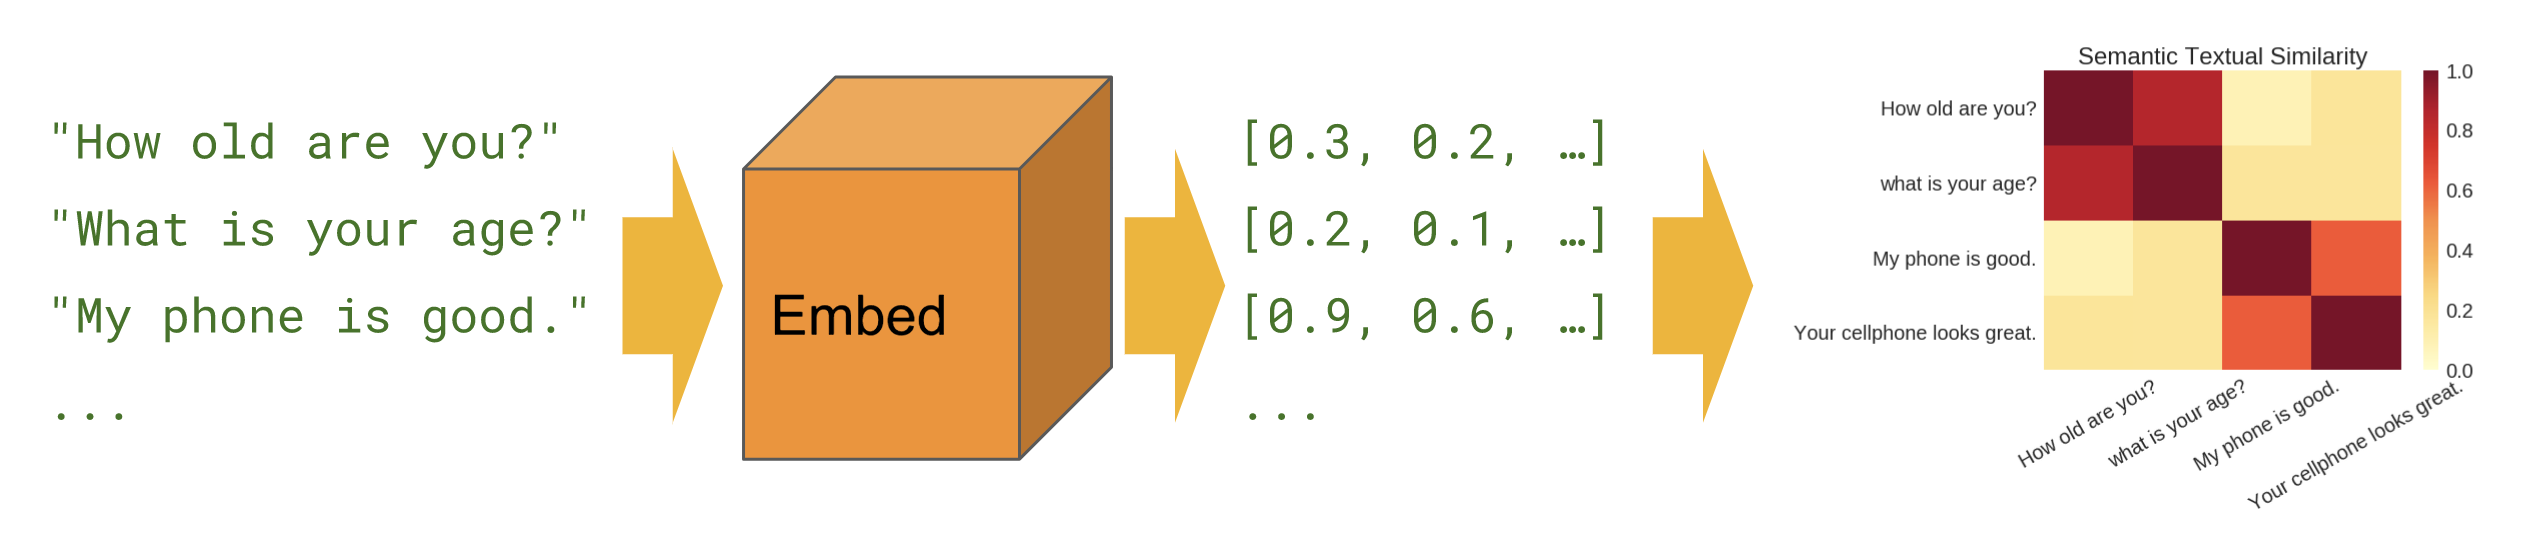
\includegraphics [scale=0.33]{Figure/use.png}
    \caption{Esempio funzionamento Universal Sentence Encoder: le frasi vengono trasformate in vettori a lunghezza fissa, per valutarne la similarità si può banalmente calcolare l'inner-product di tutte le coppie e mostrarlo in una matrice.}
    \label{fig:my_label}
\end{figure}
\FloatBarrier
In questo lavoro, è stato usato il multilingual Universal Sentence Encoder per effettuare l'embedding di frasi scritte in linguaggio naturale al fine di addestrare un classificatori in grado di riconoscere i topic a cui appartiene la frase e dei classificatori in grado di riconoscere la sensibilità della frase appartenente al topic.

%%%%%%%%%%%%%%%%%%%%%%%%%%%%
\chapter{Related Work}
Qui ci va quell'articolo che abbiamo trovato su PET passo passo illustrato, e sottolineato i pregi/difetti.

%%%%%%%%%%%%%%%%%%%%%%%%%%%%
\chapter{Metodologia}
\label{ch:method}
L'obiettivo di questo lavoro è dotare Knoxly di un modulo intelligente capace di comprendere la semantica di un testo scritto in linguaggio naturale (\textit{il testo parla di argomenti potenzialmente sensibili?}), comprendere se il testo che si sta per divulgare sul Web contiene dati sensibili o personali~\cite{dataSpectrum} (\textit{l'utente sta divulgando la propria opinione politica?}), inviare - nel caso - una notifica all'utente (privacy awareness), ed adattarsi alle esigenze dell'utente (alcuni utenti, es. esercenti fisici, potrebbero non essere interessati a ricevere notifiche riguardo la possibile divulgazione della loro location). Alla luce degli obiettivi, ci si è mossi verso tecniche basate su Intelligenza Artificiale che si sono mostrate utili in svariati contesti simili (si faccia riferimento, ad esempio, a~\cite{dontTweetThis, hybrid}).

\begin{figure}[h!t]
    \centering
    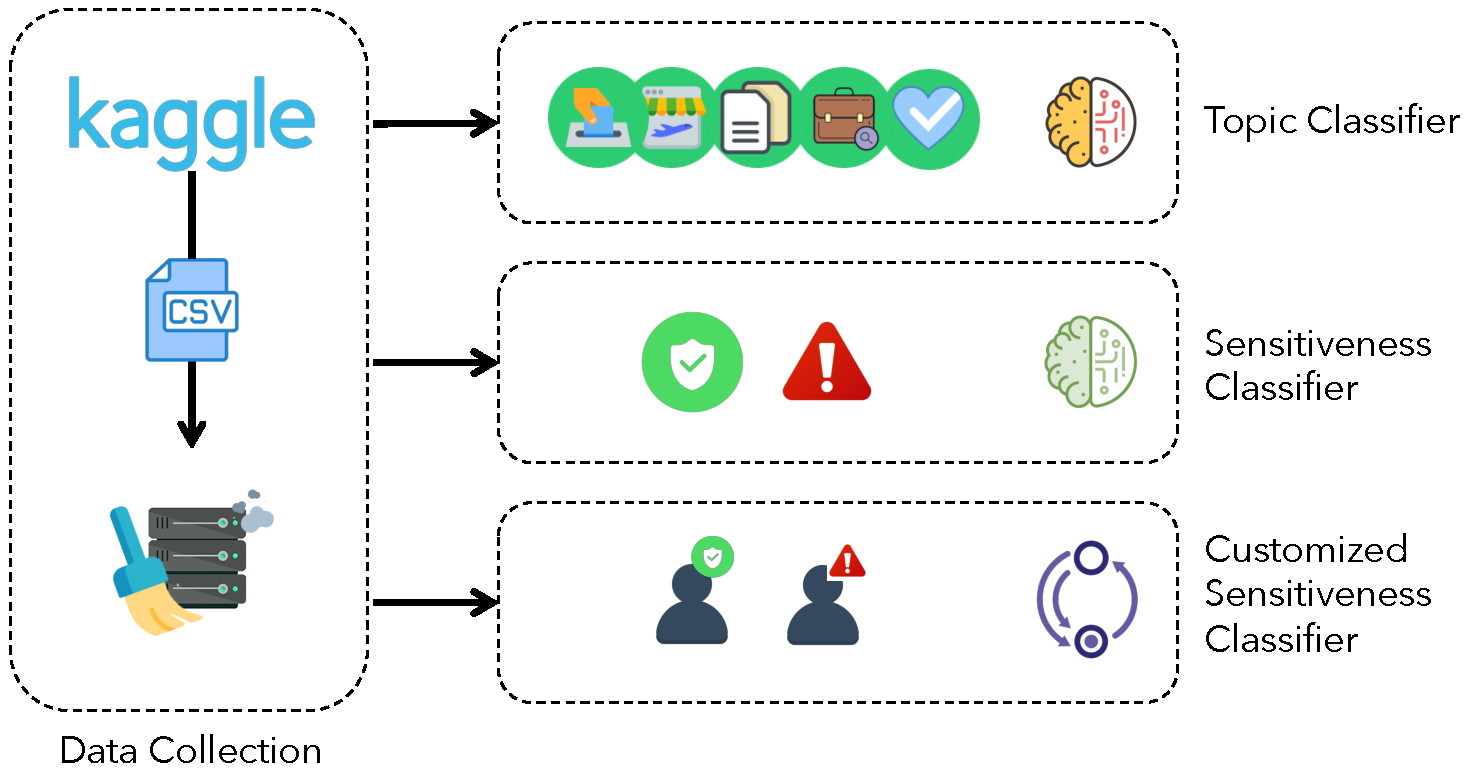
\includegraphics[width=15cm]{Figure/grafici/wholemethodology_cropped.pdf}
    \caption{Principali fasi della metodolgia adottata: (1) \textit{Data collection}, individuazione, raccolata e pre-processing dei dati utili alle fasi successive; \textit{(2) Topic classifier}, realizzare una modello che data una frase è in grado di riconoscere il topic di appartenenza; \textit{(3) Sensitiveness classifier}, realizzare un modello che data una frase è in grado di capire se contiene dati potenzialmente personali e sensibili; \textit{(4) Customized sensitiveness classifier}, realizzare un modello in grado di capire quali sono i dati sensibili per un utente adattandosi alla sua percezione di privacy.}
    \label{fig:wholemethod}
\end{figure}

Per realizzare il core intelligente di Knoxly è stata seguita una metodologia che si suddivide nelle seguenti fasi (vedi Figura~\ref{fig:wholemethod}):
\begin{itemize}
    \item Data collection (Sezione~\ref{datacollection}): individuazione, raccolta e pre-processing dei dati;
    \item Topic classifier (Sezione~\ref{sec:topicclass}): realizzare una modello che data una frase è in grado di riconoscere il topic di appartenenza;
    \item Sensitiveness classifier (Sezione~\ref{sec:sensclass}): realizzare un modello che data una frase è in grado di capire quanto essa sia sensibile;
    \item Customized sensitiveness classifier (Sezione~\ref{sec:pres_sens_class}): realizzare un modello in grado di capire quali siano i dati sensibili per un utente.
\end{itemize}



\section{Data collection}
\label{datacollection}
La prima fase del lavoro consiste nel collezionare i dati utili agli step successivi. Per creare il dataset su cui verranno addestrati i modelli di (a) \textit{Topic classifier}, (b) \textit{Sensitiveness classifier} e (c) \textit{customized sensitiveness classifier}, bisogna come prima cosa raccogliere i dati raw (non elaborati).
Sulla base di quanto spiegato nella sezione~\ref{ssec:sensitive_data} sono stati individuati quattro topic di particolare interesse: politica, viaggi, salute, lavoro, come fatto anche in~\cite{looseTweets,dontTweetThis,MalandrinoScarano}.

\begin{table}[h]

\centering
    \fontsize{4.6mm}{4.6mm}\selectfont{
    \renewcommand{\arraystretch}{1.4}
    \setlength\tabcolsep{4.0pt}
    \begin{tabular}{c|c|c|c}
    \toprule
    \textbf{Topic} & \textbf{nome dataset} & \textbf{Reference} & \textbf{\# entry} \\
    \midrule
    Politics & Election Day Tweets & \cite{ds_pol}  & 393.764 \\ \hline
    Health & Medical Transcriptions & \cite{ds_health1} & 2.348 \\ \hline
    Health & Medical Speech, Transcription, and Intent & \cite{ds_health2} & 706 \\ \hline
    Job & AMAZON Job Skills & \cite{ds_job} & 2.505 \\ \hline
    Travel & Twitter US Airline Sentiment & \cite{ds_travel} & 14.427 \\ \hline
    General & The Movies Dataset & \cite{ds_general} & 44.306 \\
    \bottomrule
    \end{tabular}
    }
\caption{Dataset scelti su Kaggle.com per ogni topic d'interesse.}
\label{tab:ds_scelti}
\end{table}
\FloatBarrier

Una volta definiti i topic, sono stati individuati dei dataset opportuni. In particolare, è stato effettuato il download di dataset messi a disposizione dal sito \href{https://www.kaggle.com/}{kaggle.com} i quali dopo una fase di pre-processing sono stati uniti in un unico \quotes{dataset raw}. Nella tabella~\ref{tab:ds_scelti} vengono mostrati i dataset selezionati per ogni topic con il relativo numero di elementi e il link per scaricarlo.

Si è deciso di introdurre un topic che chiameremo \quotes{General} il quale ci servirà per aumentare l'eterogeneità dei dati, creando rumore. È chiaro che un modello di machine learning basato solo sui topic potenzialmente ricchi di dati sensibili e personali, classificherebbe qualsiasi testo in una delle categorie individuate: ciò genererebbe misclassification perchè esistono dei testi che non ricadono in nessuna delle categorie tra health, politics, job e travel. Nel topic \quotes{General} sono contenute delle trame di film: sono state scelte le trame perchè queste sono composte da testi brevi e raccontano una storia e in alcuni casi questa può riportare dei dati sensibili e personali riguardo i personaggi.

I dataset scelti sono salvati come file {\tt .csv}: essi presentano diverse colonne, alcune di queste irrilevanti ai fini di questo lavoro.

\begin{table}[h!t]
\centering
\begin{tabular}{|l|c|l|}
\hline
\multicolumn{1}{|c|}{\textbf{Topic}} & \textbf{file} & \multicolumn{1}{c|}{\textbf{col. scelta}} \\ \hline
Politics & {\tt election\_day\_tweets.csv} & text \\ \hline
Health & {\tt mtsamples.csv} & description \\ \hline
Health & {\tt overview-of-recordings.csv} & phrase \\ \hline
Job & {\tt amazon\_jobs\_dataset.csv} & \begin{tabular}[c]{@{}l@{}}description,\\ basic qualifications,\\ preferred qualifications\end{tabular} \\ \hline
Travel & {\tt Tweets.csv} & text \\ \hline
General & {\tt movie\_metadata.csv} & overview \\ \hline
\end{tabular}
\caption{File e colonne (col. scelta) selezionate dai dataset di Kaggle}
\label{tab:col_scelte}
\end{table}
\FloatBarrier

In Tabella~\ref{tab:col_scelte} si elencano i file scelti e le colonne selezionate che comporranno il dataset.

\section{Pre-processing sui raw data}
\label{sec:preprocessingraw}
I testi selezionati risultano molto eterogenei quindi prima di raggruppare tutto in un unico dataset è stata necessaria una \quotes{pulizia} di questi dati.

Dai vari subset ricavati dai dataset originali di Kaggle sono state eliminate le righe che contenevano un testo di lunghezza $l<3$ caratteri e che non erano scritti in lingua inglese. La fase language detection è stata condotta utilizzando la libreria Python  TextBlob\footnote{\url{https://textblob.readthedocs.io/en/dev}}.

Si è notato che i testi nel dataset Job risultano essere particolarmente lunghi (lunghezza media degli annunci è di 968 caratteri, SD=788.40) e ciò può rappresentare un problema di conformità rispetto gli altri dataset considerati. Per ridurre le dimensioni delle singole entry appartenti alla categoria job si è deciso di dividere in varie parti l'annuncio di lavoro. Questa operazione è stata eseguita utilizzando il sentence splitter\footnote{\url{https://github.com/berkmancenter/mediacloud-sentence-splitter}}, fornito dai ricercatori Philipp Koehn e Josh Schroeder~\cite{Koehn07}. 

Terminata questa fase, i vari dataset processati sono pronti per essere uniti ed etichettati.

\section{Topic classification}
\label{sec:topicclass}
Il primo obiettivo del lavoro è la definizione ed implementazione di un modulo intelligente capace di comprendere la semantica di un testo scritto in linguaggio naturale, che sia in grado di capire di cosa l'utente sta parlando.

\begin{figure}[h!t]
    \centering
    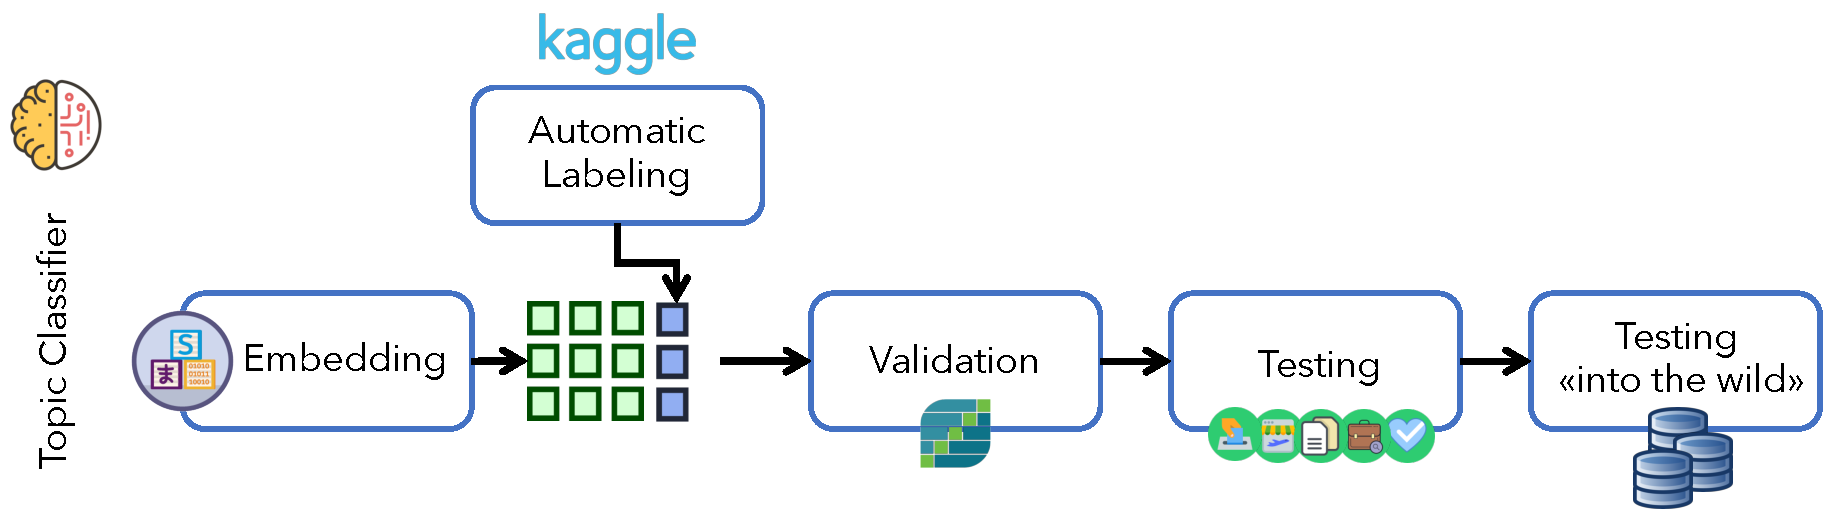
\includegraphics[width=15cm]{Figure/grafici/topicmethod_cropped.pdf}
    \caption{Principali fasi per la creazione del modulo Topic Classifier: (\textit{Embedding}) le frasi dei vari dataset vengono trasformate in vettori a lunghezza fissa; (\textit{Automatic Labeling}) in base al dataset di provenienza ciascun sample (embedding) viene etichettato automaticamente; (\textit{Validation}) mediante una k-fold cross-validation si validano vari classificatori basati sul supervised learning e si effettua il tuning degli iper-parametri utilizzando il training set $trs$; (\textit{Testing}) una volta ottenuti i migliori parametri per ciascun classificatore, si effettua il testing sul test set $tss$; (\textit{Testing \quotes{into the wild}}) si effettua un ulteriore testing su nuovi dati.}
    \label{fig:topicmethod}
\end{figure}

A tal fine è stata seguita una metodologia che consta nelle seguenti fasi (vedi Figura~\ref{fig:topicmethod}):
\begin{itemize}
    \item Creazione del dataset (Sezione~\ref{ssec:createds}): si illustra (a) la/e tecnica/che utilizzate per la conversione dei testi del dataset in vettori di numeri reali (sample) da dare in input al classificatore, (b) la strategia di labeling dei sample; 
    \item Validation (Sezione~\ref{ssec:validation_Topic}): validazione del modello realizzato utilizzando la k-fold cross-validation;
    \item Testing (Sezione~\ref{ssec:testing_Topic}): testing delle performance del metodo sul test set;
    \item Testing~\quotes{into the wild} (Sezione~\ref{ssec:testing_wild}): ulteriore testing delle performance del metodo, su un dataset molto più ampio.
\end{itemize}

\subsection{Creazione del dataset}
\label{ssec:createds}
Una volta ultimata la fase di pre-processing i dati sono stati uniti in unico dataset composto da 2426861 elementi. Per questo esperimento abbiamo deciso di utilizzare un subset di questo dataset, composto da 1000 elementi per ciascun topic, selezionati con una funzione {\tt random}. Successivamente si è passati alla fase di rappresentazione del testo (Sezione~\ref{sssec:rappresentazione}) e labeling (Sezione~\ref{sssec:textlabeling}).

\subsubsection{Rappresentazione del testo}
\label{sssec:rappresentazione}
Per rappresentare i testi è stato utilizzato USE di Google (vedi Sezione~\ref{sec:use}), perchè si ipotizza che le frasi appartenenti allo stesso topic siano simili fra loro e di conseguenza anche i vettori risultanti dall'operazione di embedding saranno simili. Ogni testo viene quindi convertito in un array di 512 elementi. Per mostrare la validità di questa ipotesi è stato selezionato un campione {\tt random} di 5 frasi per ogni topic, è stato effettuato l'embed delle frasi e poi calcolato l'inner product degli embed. L'inner product è una tecnica molto semplice per comprendere la similarità tra due vettori. Il valore di similarità $s \in [0..1]$, dove $1$ indica frasi / vettori identiche / ci, $0$ indica completa dissimilarità, quindi più il valore è vicino a $1$ più le / i frasi / vettori sono simili.

Di seguito vengono mostrate le matrici di similarità ottenute dell'inner product. Si può notare che le matrici di similarità con i valori più alti sono politics (Figura~\ref{fig:mtrsim_p}) - con valori che vanno da 0.63 a 1 -, job (Figura~\ref{fig:mtrsim_j}) - con valori che vanno da 0.72 a 1.

Infine, è stata realizzata una matrice che mette insieme le frasi selezionate per ciascun topic per valutare quanto queste se appartenenti a diversi topic si somiglino (differiscano tra loro in questo caso). Il risultato è mostrato in Figura~\ref{fig:mtrsim_mix} dove si può notare che le celle colorate con toni chiari (valori superiori a 0.5) siano ottenute dalla intersezione di frasi appartenenti allo stesso topic, mentre, le celle colorate con toni scuri (valori inferiori al 0.5) siano date dell'inner product di frasi appartenenti a topic diversi.

\begin{figure}[h!t]
    \centering
    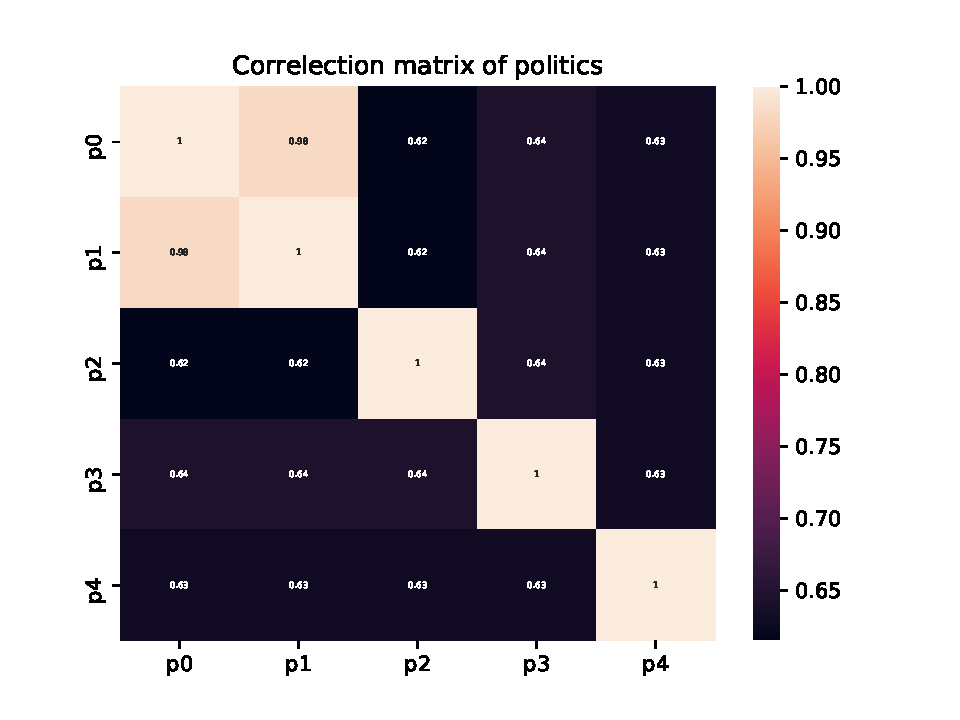
\includegraphics{Figure/simMatr/politics.pdf}
    \caption{matrici di similarità delle frasi appartenenti al topic politics}
    \label{fig:mtrsim_p}
\end{figure}
\FloatBarrier

\begin{figure}[h!t]
    \centering
    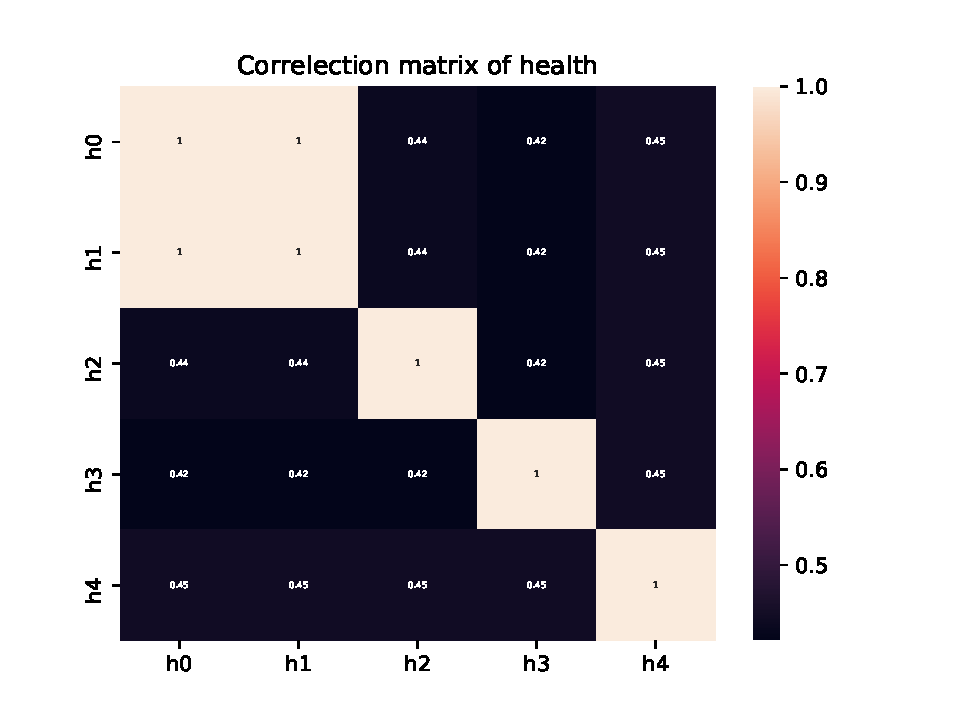
\includegraphics{Figure/simMatr/health.pdf}
    \caption{matrici di similarità delle frasi appartenenti al topic health}
    \label{fig:mtrsim_h}
\end{figure}
\FloatBarrier

\begin{figure}[h!t]
    \centering
    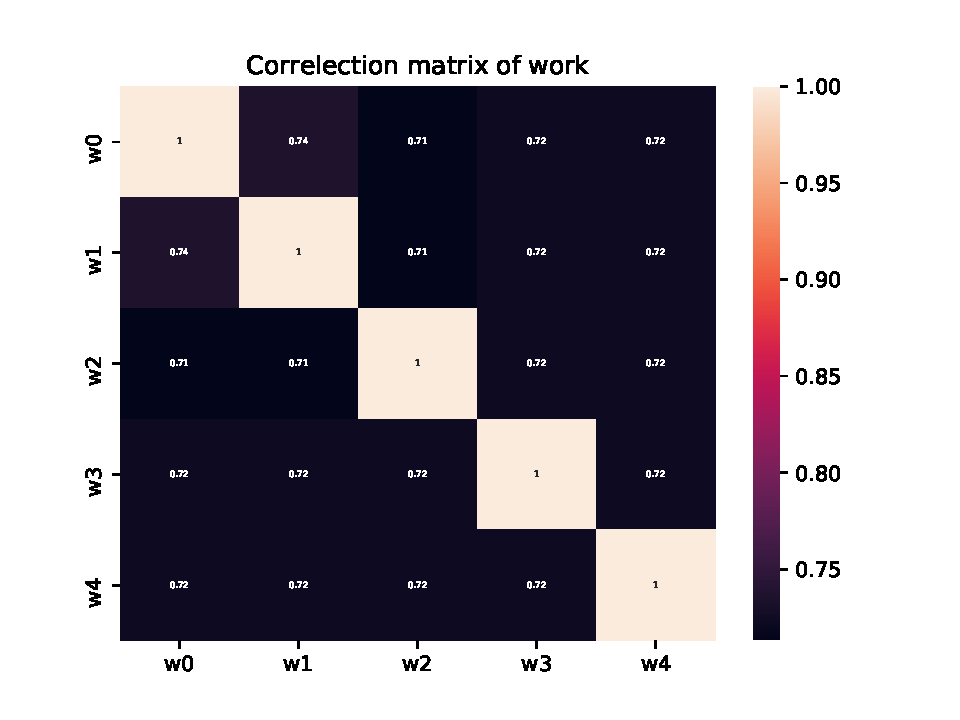
\includegraphics{Figure/simMatr/work.pdf}
    \caption{matrici di similarità delle frasi appartenenti al topic job}
    \label{fig:mtrsim_j}
\end{figure}
\FloatBarrier

\begin{figure}[h!t]
    \centering
    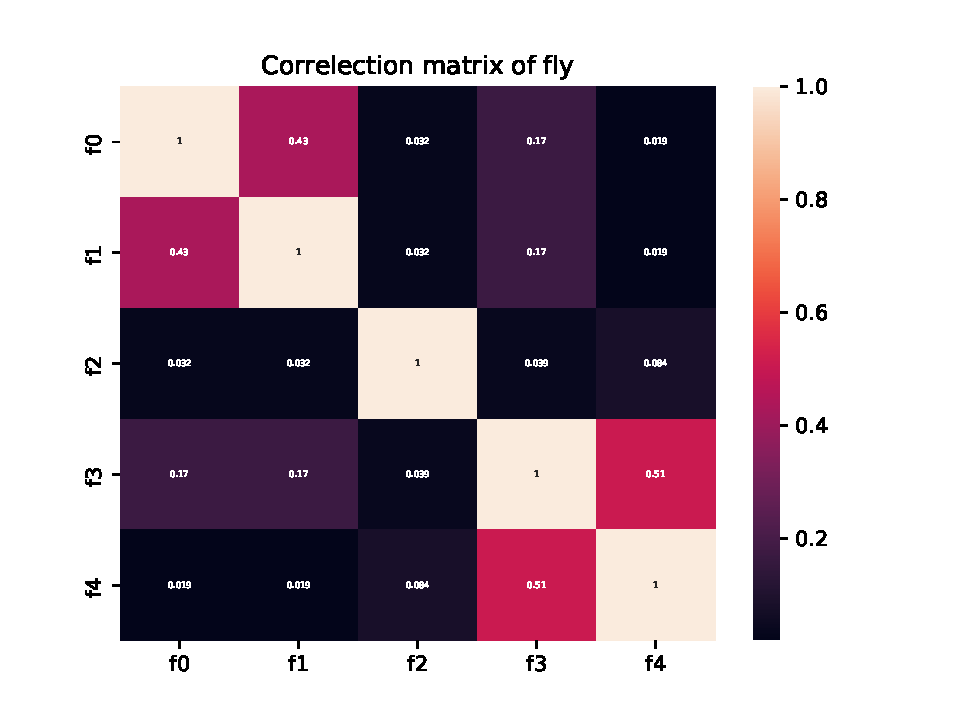
\includegraphics{Figure/simMatr/fly.pdf}
    \caption{matrici di similarità delle frasi appartenenti al topic travel}
    \label{fig:mtrsim_t}
\end{figure}
\FloatBarrier

\begin{figure}[h!t]
    \centering
    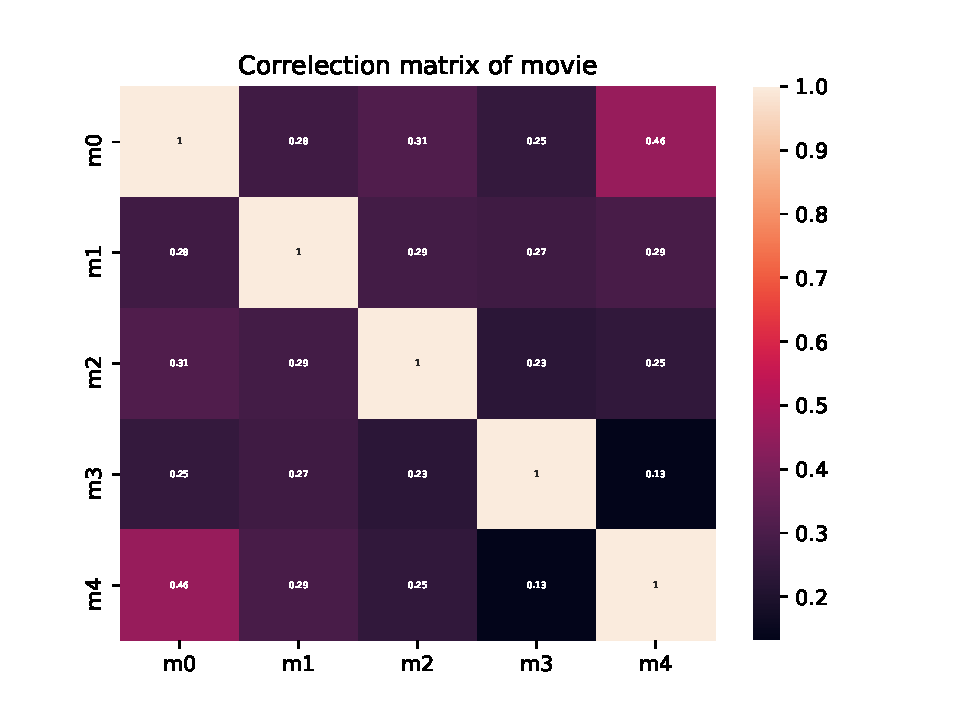
\includegraphics{Figure/simMatr/movie.pdf}
    \caption{matrici di similarità delle frasi appartenenti al topic general}
    \label{fig:mtrsim_g}
\end{figure}
\FloatBarrier

\begin{figure}[h!t]
    \centering
    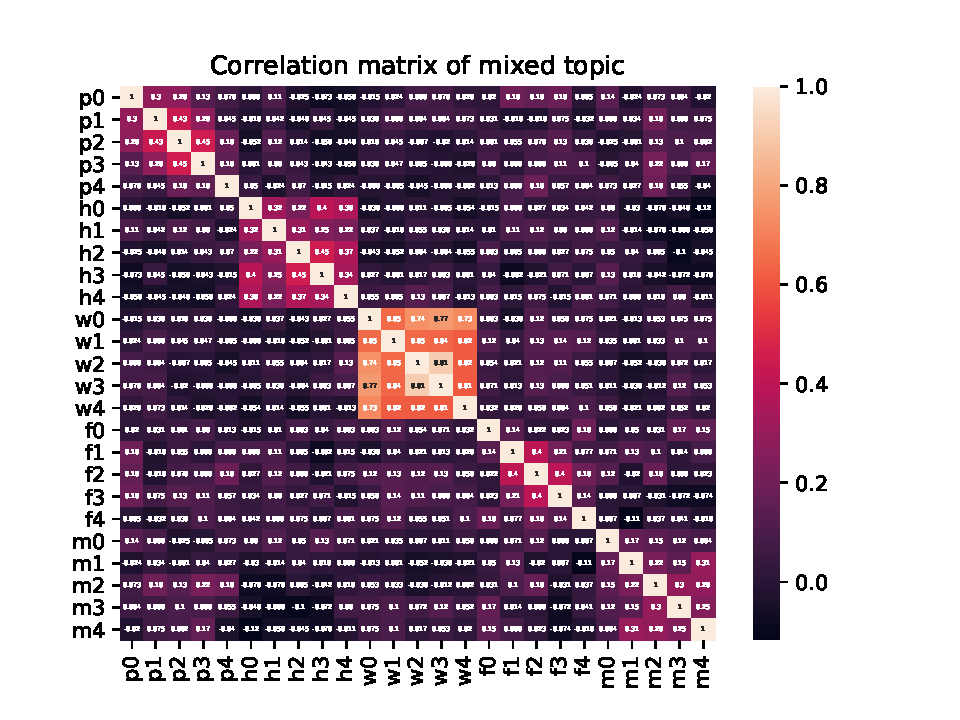
\includegraphics{Figure/simMatr/mixed.pdf}
    \caption{matrici di similarità delle frasi appartenenti ai diversi topic}
    \label{fig:mtrsim_mix}
\end{figure}
\FloatBarrier

\subsubsection{Text labeling}
\label{sssec:textlabeling}
Dopo aver rappresentato efficacemente il dataset di testi scritti in linguaggio naturale, si è passati alla fase di labeling, che consiste nell'assegnazione di una classe di appartenenza a ciascun sample. In questo caso, l'operazione è automatica in quanto i sample sono già implicitamente etichettati, in base al dataset da cui provengono. In Tabella~\ref{tbl:mtc} è mostrata la logica di labeling.


\begin{table}[h!t]
\centering
\begin{tabular}{c|c|c}
\toprule
\textbf{Topic} & \textbf{\# sample} & \textbf{Label} \\ \midrule
Politics & 1000 & 0 \\ 
Health & 1000& 1 \\ 
Job & 1000& 2 \\ 
Travel & 1000& 3 \\ 
General & 1000& 4 \\ \bottomrule
\end{tabular}
\caption{Logica di conversione da topic a etichette 
numeriche e informazioni dataset.}
\label{tbl:mtc}
\end{table}

\subsection{Validation}
\label{ssec:validation_Topic}
Inizialmente abbiamo diviso il dataset in Tabella~\ref{tbl:mtc} in un 80\% riservato al training ed un 20\% riservato al testing attraverso la funzione {\tt train\_test\_split} (\textit{stratified}) di scikit-learn\footnote{\url{https://scikit-learn.org/stable/}} per Python.

È stata effettuata una fase di validation sfruttando il training set. In particolare si è adoperata la \textbf{k-fold} cross-validation, una procedura di resampling utilizzata per valutare modelli di machine learning su un campione di dati limitato. La procedura ha come unico parametro \textit{k} che rappresenta il numero di quanti subset si devono creare partendo dal campione originale, nel nostro caso $ k = 5 $.

Tale fase è stata sfruttata anche per l'hyper-parameter tuning usando il metodo {\tt GridSearchCV} di scikit-learn per Python.

In questo lavoro è stato utilizzato uno dei più popolari modelli di machine learning disponibile in letteratura e implementato in scikit-learn, esso è il Random Forest(Sezione~\ref{ssec:RF}). Le sue prestazioni si basano principalmente sul \textit{numero di stimatori}, quindi abbiamo testato da 20 a 1000 stimatori. I migliori risultati sono stati trovati tra 100 e 550 stimatori.

In questa fase si è tentato di massimizzare il parametro F-score (vedi Sezione~\ref{metrics}), impostando oppurtunamente {\tt scoring} di {\tt GridSearchCV}.

\begin{table}[h]
\centering
\begin{tabular}{|c|c|c|}
\hline
\textbf{\# estimatori} & \textbf{Variazione} & \textbf{Risultato} \\ \hline
17 & +/-0.012 & 0.948 \\ \hline
37 & +/-0.010 & 0.963 \\ \hline
51 & +/-0.009 & 0.965 \\ \hline
177 & +/-0.006 & 0.966 \\ \hline
213 & +/-0.006 & 0.968 \\ \hline
517 & +/-0.005 & 0.966 \\ \hline
\end{tabular}
\caption{risultati ottenuti dalla fase di validation}
\label{tab:validationresult}
\end{table}
\FloatBarrier

\subsection{Testing}
\label{ssec:testing_Topic}
Una volta ottenuti i migliori parametri per ciascun classificatore abbiamo valutato le loro performance sul dataset di testing.

La tabella~\ref{tbl:training_ds1000} riporta le performance ottenute da ciascun classificatore sul testing set.
\begin{table}[h]
\begin{tabular}{|l|l|c|c|c|c|c|}
\hline
\multirow{2}{*}{\textbf{Classifier}} & \multirow{2}{*}{\textbf{Metric}} & \multicolumn{5}{c|}{\textbf{Topics}} \\ \cline{3-7} 
 &  & Politics & Health & Job & Travel & General \\ \hline
\multirow{4}{*}{RF} & Accuracy & \multicolumn{5}{c|}{0.983} \\ \cline{2-7} 
 & Precision & 0.979 & 0.99 & 0.985 & 0.966 & 0.994 \\ \cline{2-7} 
 & Recall & 0.965 & 0.995 & 0.985  & 0.995 & 0.975 \\ \cline{2-7} 
 & Fscore & 0.972 & 0.992 & 0.985 & 0.980 & 0.984 \\ \hline
\end{tabular}
\caption{Risultati per la fase di testing di Random Forest sul dataset ds1000.csv}
\label{tbl:training_ds1000}
\end{table}
\FloatBarrier
Si ricorda che l'obiettivo di questo step è di sviluppare un metodo per riconoscere il topic d'appartenenza di un testo scritto in linguaggio naturale con riferimento ai quattro topic più citati nella letteratura sulla privacy\cite{looseTweets,dontTweetThis}, più un topic generico. In particolare, si vuole avere un classificatore capace di ottenere buone prestazioni su tutte le classi individuate. 

Il \textit{TopicClassifier} basato su RF\ref{ssec:RF} così addestrato è stato \quotes{dumpato} in un oggetto {\tt pickle}\footnote{https://docs.python.org/3/library/pickle.html}.

\subsection{Testing \textit{into the wild}}
\label{ssec:testing_wild}
\textit{TopicClassifier} è stato oggetto di una ulteriore fase di testing. Si è pensato di misurare le performance del classificatore su un dataset molto più ampio, rinominato \quotes{wild dataset}. Wild dataset è composto da 2000 elementi per ciascun topic/categoria (politics, health, job, travel e general) non appartenenti al dataset di addestramento nè a quello di testing precedentemente visto.

La tabella~\ref{tbl:testing_wild} riporta le misure ottenute dalla sperimentazione \textit{into the wild} di \textit{TopicClassifier}. 
\begin{table}[h]
\begin{tabular}{|l|l|c|c|c|c|c|}
\hline
\multirow{2}{*}{\textbf{Classifier}} & \multirow{2}{*}{\textbf{Metric}} & \multicolumn{5}{c|}{\textbf{Topics}} \\ \cline{3-7} 
 &  & Politics & Health & Job & Travel & General \\ \hline
\multirow{4}{*}{RF} & Accuracy & \multicolumn{5}{c|}{0.988} \\ \cline{2-7} 
 & Precision & 0.992 & 0.995 & 0.985 & 0.975 & 0.993 \\ \cline{2-7} 
 & Recall & 0.969 & 0.995 & 0.993 & 0.996 & 0.988 \\ \cline{2-7} 
 & Fscore & 0.980 & 0.995 & 0.989 & 0.985 & 0.999 \\ \hline
\end{tabular}
\caption{Risultati della fase di testing sul dataset wild}
\label{tbl:testing_wild}
\end{table}
\FloatBarrier
\textit{TopicClassifier} durante l'esperimento \textit{into the wild} mostra delle performace simili a quelle ottenute durante la fase di testing (Sezione~\ref{ssec:testing_Topic}), ragion per cui si può affermare di aver effettuato una fase di training efficace.

\section{Sensitivity classification}
\label{sec:sensclass}
Una volta ottenuto un classificatore in grado di riconoscere il topic d'appartenenza di un testo scritto in linguaggio naturale con riferimento ai quattro topic più citati nella letteratura sulla privacy, più un topic generico, il focus si sposta sul capire se una data frase (appartente ad un topic specifico) contenga o meno dati sensibili e/o personali. Un esempio di testo con contenuti sensibili e non sensibili è riportato in Tabella~\ref{tbl:example_sens}.

\begin{table}[h]

\centering
\begin{tabular}{c|c|c}
\hline
\textbf{Frase} & \textbf{Topic} & \textbf{Sensibile} \\ \hline
\textit{Questa notte non ho dormito} & Health & \textbf{No} \\ \hline
\textit{Soffro di insonnia} & Health & \textbf{Sì} \\ \hline
\end{tabular}
\caption{esempio di contenuti sensibili e non}
\label{tbl:example_sens}
\end{table}
\FloatBarrier

A tal fine, è stata definita una metodologia come segue (vedi Figura~\ref{fig:methodsens}):
\begin{itemize}
    \item Creazione Dataset sensitivity (Sezione~\ref{ssec:create_sens_ds}): rappresentazione dei sample e labeling dei dati;
    \item Validation: validazione del modello realizzato usando la k-fold cross-validation;
    \item Testing: testing delle performance del metodo sul test set.
\end{itemize}

\begin{figure}[h!t]
    \centering
    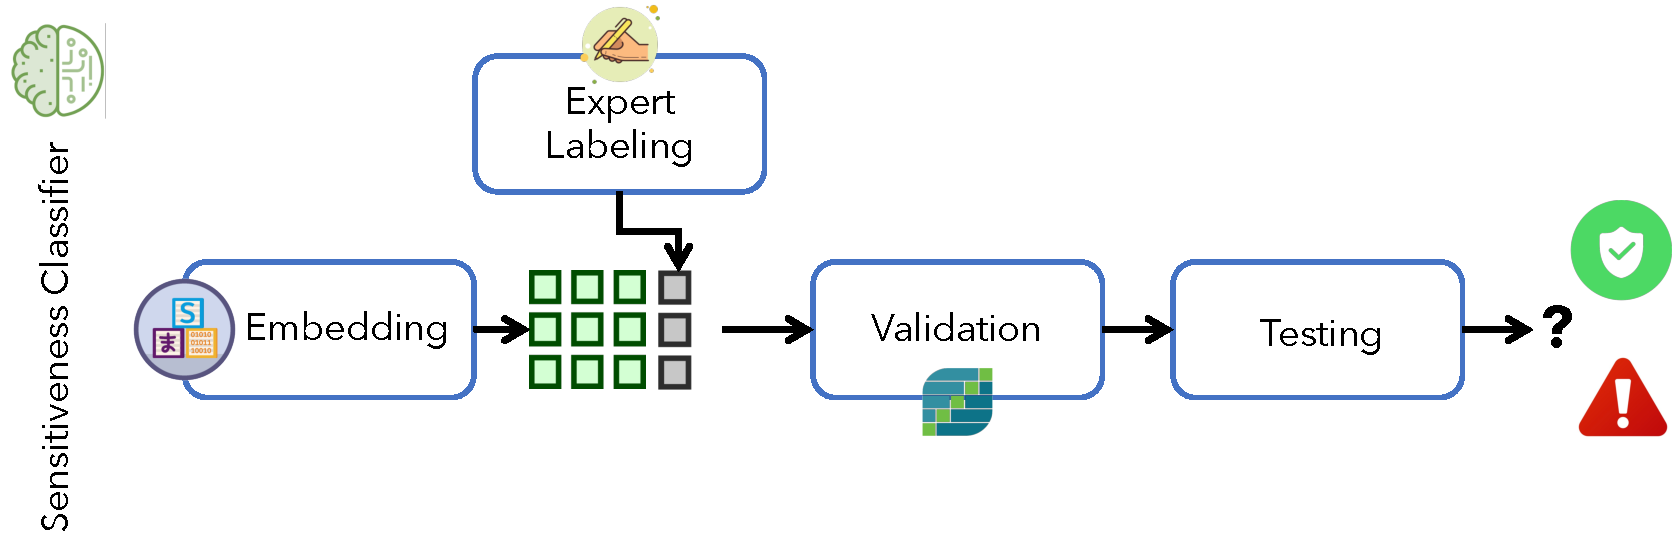
\includegraphics[width=15cm]{Figure/grafici/sensitivenessmethod_cropped.pdf}
    \caption{Principali fasi per la creazione del modulo Sensitiveness classifier: (\textit{Embedding}) le frasi dei vari dataset vengono trasformate in vettori a lunghezza fissa; (\textit{Expert labeling}) tramite una serie di regole ben definite~\cite{}, un esperto del dominio effettua manualmente il labeling dei sample; (\textit{Validation}) mediante una k-fold cross-validation si validano vari classificatori basati sul supervised learning e si effettua il tuning degli iper-parametri utilizzando il training set $trs'$; (\textit{Testing}) una volta ottenuti i migliori parametri per ciascun classificatore, si effettua il testing sul test set $tss'$;   }
    \label{fig:methodsens}
\end{figure}

\subsection{Creazione Dataset sensitivity}
\label{ssec:create_sens_ds}
Per la creazione di questo dataset abbiamo riutilizzato parte del {\tt ds1000.csv} precedentemente creato per la fase di Topic Classification~\ref{tbl:training_ds1000}. In particolare abbiamo selezionato con una funzione {\tt random} 200 elementi per ciascuna categoria di riferimento.

\begin{table}[h!t]
    \centering
    \begin{tabular}{c|c|c}
    \hline
        \textbf{Topic} & \textbf{ID} & \textbf{\# entry} \\ \hline
        Politics & 0 & 200 \\ \hline
        Health & 1 & 200 \\ \hline
        Job & 2 & 200 \\ \hline
        Travel & 3 & 200 \\ \hline
        General & 4 & 200 \\ \hline
    \end{tabular}
    \caption{ds200.csv, il dataset da 200 elementi per topic}
    \label{tab:ds200.csv}
\end{table}
\FloatBarrier

\subsubsection{Sensitiveness labeling}
\label{sssec:sens_labeling}
In questa fase ds200.csv è stato etichettato secondo le regole delineate in~\cite{dataSpectrum}.
\begin{figure}
    \centering
    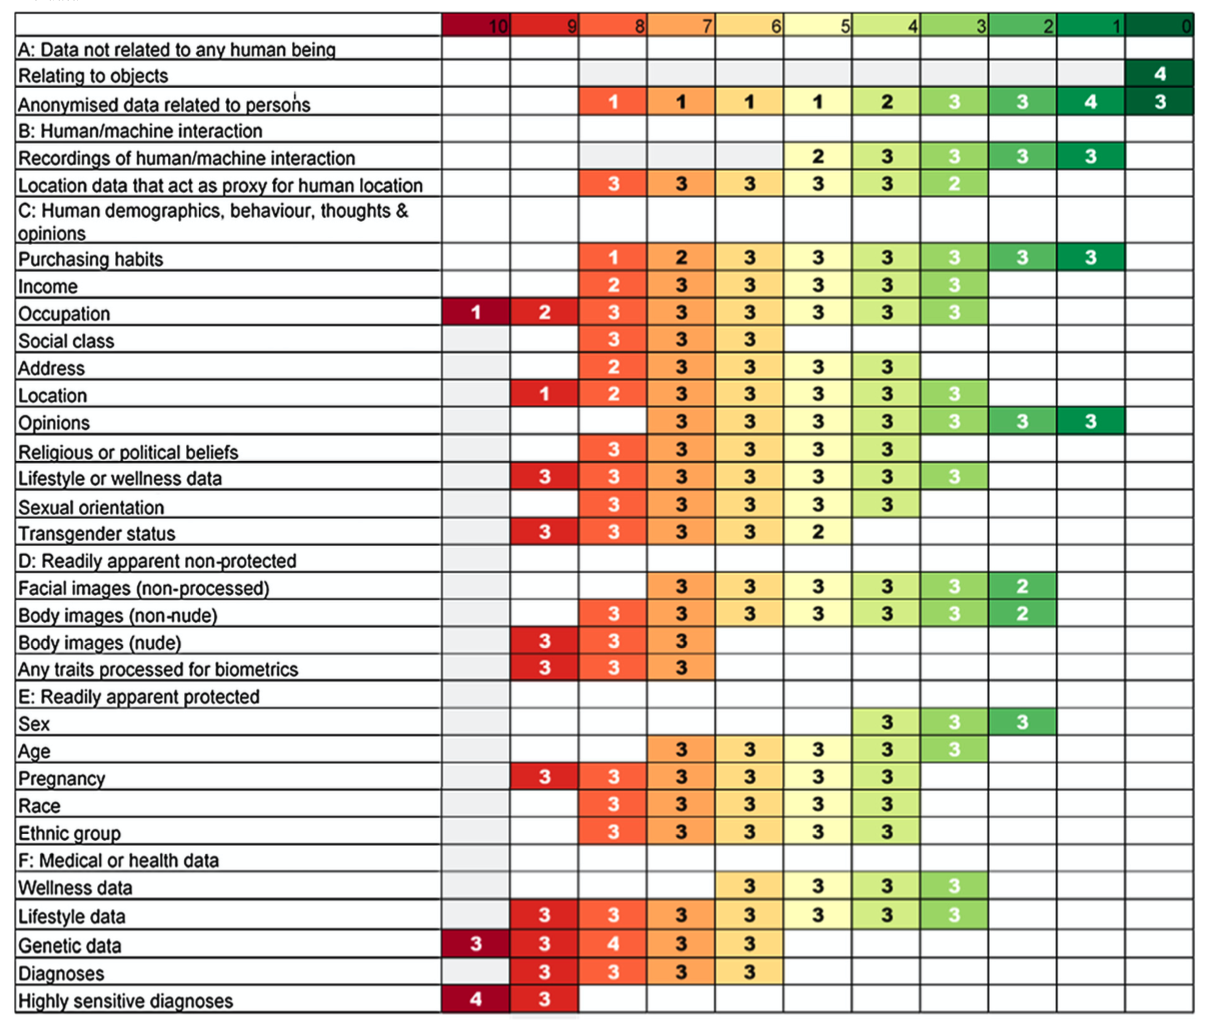
\includegraphics[scale=0.4]{Figure/sensTbl.png}
    \caption{Tabella delle sensibilità utilizzata da Rumbold et al.~\cite{spectrum}}
    \label{fig:sensRumboldd}
\end{figure}
\FloatBarrier
Le righe della tabella mostrate in figura~\ref{fig:sensRumboldd} contengono la categoria a cui una frase può appartenere e quanto essa possa essere sensibile, il \textbf{livello di sensibilità} varia da 0 (non sensibile) a 10 (molto sensibile). I numeri presenti nelle celle variano da 0 a 4 ed essi rappresentano la \textbf{frequenza} che l'argomento descritto nella riga si presenti con il livello di sensibilità descritto nella colonna. Ad esempio prendiamo l'argomento \textit{Relating to object} esso ha un livello di sensibilità pari a 0 e nella cella viene riportato il numero 4, questo vuol dire che quando si parlerà di argomenti relativo ad oggetti questi saranno sicuramente poco sensibili.


%\subsubsection{Tabella delle sensibilità}
%\label{ssec:tblSens&Euricstic}
In accordo allo studio fatto da Rumbold et al.~\cite{dataSpectrum} è stata definita una tabella delle sensibilità a cui fare riferimento per determinare se un contenuto va etichettato come sensibile (1) o meno (0). I criteri definiti nella tabella~\ref{tbl:senstbl} sono stati ottenuti utilizzando il seguente metodo.

Si definiscono $freq$ i valori di frequenza utilizzati da Rumbold et al. Sia $freq[i]$ il valore di frequenza per il livello di sensibilità $i$, $i\in[0..10]$.

I livelli $i<5$ indicano basso grado di sensibilità, viceversa i livelli $i>=5$ indicano alto grado di sensibilità. 

Calcoliamo quindi lo score totale di sensibilità come

$\sum^{N}_{i=x}freq[i]$, $N=4,10$, $x=0,5$. 

Etichettiamo un elemento non sensibile se:
\begin{equation}
\sum^{4}_{i=0}freq[i] > \sum^{10}_{i=5}freq[i]
\end{equation}

Viceversa, se sensibile.

Informalmente, si confronta la somma delle frequenze che hanno un livello di sensibilità compreso fra $0$ e $4$ con la somma delle frequenze che hanno un livello di sensibilità compreso fra $5$ e $10$. Se la somma delle frequenze che hanno un livello di sensibilità compreso fra $5$ e $10$ è maggiore rispetto alla somma delle frequenze che hanno un livello di sensibilità compreso fra $0$ e $4$ allora l'argomento risulta essere sensibile e i testi che appartengono a tale argomento verranno etichettati con $1$, $0$ altrimenti.

\begin{table}[h]
\centering 
\begin{tabular}{|l|c|}
\hline
\multicolumn{1}{|c|}{\textbf{Regole}} & \textbf{Sensibile} \\ \hline
Dati relativi ad oggetti & \xmark \\ \hline
Dati anonimizzati relativi a persone & \xmark \\ \hline
Dati relativi ad interazioni uomo-macchina & \xmark \\\hline
Dati relativi a posizione di uomini & \cmark \\ \hline
Dati relativi ad abitudini di acquisto & \xmark \\\hline
Dati relativi allo stipendio & \cmark \\ \hline
Dati relativi al lavoro svolto & \cmark \\ \hline
Dati relativi alla propria classe sociale & \cmark \\ \hline
Indirizzo o luogo & \cmark \\ \hline
Chiara opinione religiosa o politica & \cmark \\ \hline
Altri tipi di opinioni & \xmark \\\hline
Dati sul lifestyle & \cmark \\ \hline
Orientamento sessuale & \cmark \\ \hline
Sesso in generale & \xmark \\ \hline
Dati relativi alla gravidanza & \cmark \\ \hline
Dati relativi al gruppo etnico & \cmark \\ \hline
Dati medici o stato di salute & \cmark \\ \hline
\end{tabular}
\caption{Regole per effettuare il labeling manuale. \cmark indica che una frase contenente quel dato è sensibile, \xmark viceversa.}
\label{tbl:senstbl}
\end{table}
\FloatBarrier

Una volta completata l'etichettatura abbiamo ottenuto un certo numero di testi sensibili per ogni topic. I principali dati di riferimento per questo dataset sono riportati nella tabella~\ref{tbl:ds200}.

\begin{table}[h]
\centering
\begin{tabular}{|c|c|c|}
\hline
\textbf{Topic} & \textbf{\# entry} & \textbf{\# entry sensibili} \\ \hline
Politics & 200 & 100 \\ \hline
Health & 200 & 100 \\ \hline
Job & 200 & 80 \\ \hline
Travel & 200 & 100 \\ \hline
General & 200 & 100 \\ \hline
Totale & 1000 & 480 \\ \hline
\end{tabular}
\caption{ds200.csv}
\label{tbl:ds200}
\end{table}
\FloatBarrier

\subsection{Approcci per l'analisi di sensitività}
\label{ssec:approcci}
Per analizzare il livello di sensitività di una frase abbiamo individuato due possibili tecniche mostrate in figura~\ref{fig:approccisens}:
\begin{enumerate}
    \item realizzare un singolo classificatore che è addestrato per riconoscere ed individuare se una frase contiene dati sensibili/personali o meno sull'intero dataset {\tt ds200.csv};
    \item realizzare 5 classificatori diversi, uno per ciascun topic, capaci di riconoscere ed individuare se una frase che parla di un certo argomento (cioè che appartiene ad uno dei topic di cui alla Sezione~\ref{sssec:multiclass}) contiene dati sensibili/personali o meno.
\end{enumerate}
Date le buone performance mostrate dalla classificazione per topic effettuata con il Random Forest (Sezione~\ref{sec:topicclass}), si è scelto di utilizzare Random Forest in entrambi gli approcci.

\begin{figure}[h]
    \centering
    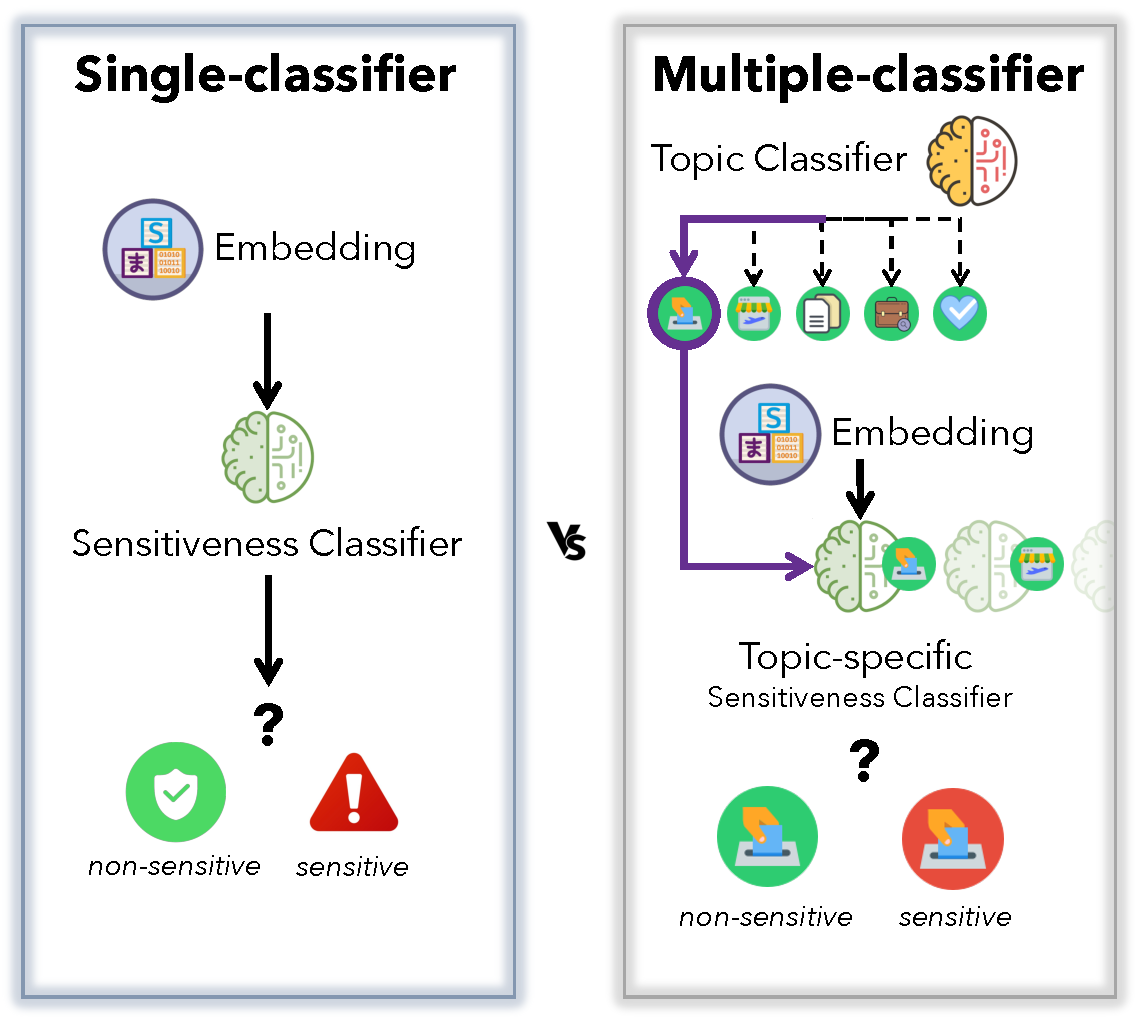
\includegraphics[width=15cm]{Figure/grafici/vs_cropped.pdf}
    \caption{I due approcci per la creazione del Sensitiveness classifier.}
    \label{fig:approccisens}
\end{figure}
\FloatBarrier



\subsubsection{Approccio con il singolo classificatore}
\label{sssec:singleclass}
Con questo approccio viene realizzato un singolo classificatore in grado di riconosce frasi contenenti dati sensibili e/o personali. Il vantaggio è quello di avere un unico classificatore sensitività in grado di individuare contenuti sensibili, lo svantaggio è il fatto che questo tipo di classificatore ha una conoscenza a grana grossa della di un dato sensibile e quindi è facile che sbagli ad assegnare il grado di sensibilità.

\paragraph{Validation} Il dataset è stato diviso in 80\% per il training e 20\% per il testing con la funzione {\tt train\_test\_split}. Il dataset di training è oggetto della validation. Abbiamo effettuato una k-fold cross-validation con $k=10$ utilizzando il metodo {\tt GridSearchCV} di scikit-learn per Python cercando di ottimizzare il roc\_auc score. In Tabella~\ref{tbl:validation_sens} si mostrano sia i parametri oggetto della funzione {\tt GridSearchCV} sia i risultati raggiunti in termini di roc\_auc score. 
\begin{table}[h]
\centering
\begin{tabular}{|c|c|c|}
\hline
\textbf{Estimatori} & \textbf{Variazione} & \textbf{Roc-AUC} \\ \hline
17 & +/-0.061 & 0.760 \\ \hline
37 & +/-0.079 & 0.783 \\ \hline
51 & +/-0.075 & 0.806 \\ \hline
177 & +/-0.076 & 0.836 \\ \hline
213 & +/-0.041 & 0.840 \\ \hline
517 & +/-0.057 & 0.847 \\ \hline
1013 & +/-0.058 & 0.851 \\ \hline
\end{tabular}
\caption{ROC AUC score ottenuti in fase di validation con Random Forest nel caso single-classifier.}
\label{tbl:validation_sens}
\end{table}
\FloatBarrier

\paragraph{Testing} Dopo la fase di validazione, sono stati ottenuti i migliori parametri per il classificatore Random Forest. Il modello viene quindi ri-addestrato sul training set e se ne misurano le performance sul test set. I risulati sono riportati in Tabella~\ref{tbl:training_sens}.

\begin{table}[h]

\centering
\begin{tabular}{|c|c|c|}
\hline
\textbf{Metric} & \textbf{Non Sensibile} & \textbf{Sensibile} \\ \hline
Accuracy & \multicolumn{2}{c|}{0.765} \\ \hline
Precision & 0.776 & 0.752 \\ \hline
Recall & 0.769 & 0.760 \\ \hline
Roc-Auc & \multicolumn{2}{c|}{0.848} \\ \hline
\end{tabular}
\caption{Performance del classificatore Random Forest ottenute nella fase di testing con approccio single-classifier.}
\label{tbl:training_sens}
\end{table}
\FloatBarrier

Matrice di confusione per questo test è mostrata in Figura~\ref{fig:mtrconf_sim_200}.


Tenuto conto della difficoltà di questo task, le performance del classificatore di sensibilità singolo sono discrete.

\subsubsection{Approccio con classificatori multipli}
\label{sssec:multiclass}
L'altro approccio al problema della sensibilità di un testo è quello di avere cinque classificatori differenti (uno per ogni topic) che verranno addestrati a riconoscere argomenti sensibili sui 200 elementi che appartengono ad ogni topic di {\tt ds200.csv}.

Di seguito sono mostrati tutti i risultati ottenuti durante la validation e il testing dei vari classificatori di sensibilità. Per esigenze di spazio, e leggibilità del documento, le matrici di confusione di ogni classificatore nella fase di testing sono state riportate in Appendice~(\ref{ch:appendix}).

\subsubsection{Validation e testing sensitiveness politics}
\label{sssec:val_testing_pol}
\paragraph{Validation} La fase di validation per ciascuno dei classificatori di sensibilità è la medesima: si suddivide il dataset in 80\% per training e 20\% per testing con la funzione {\tt train\_test\_split} di scikit-learn per Python. Il dataset di training è oggetto della validazione vera e propria che avviene con il metodo {\tt GridSearchCV} in cui si testano diversi parametri per il classificatore e si tenta di ottimizzare il roc\_auc score.  I risultati di questa fase sono riportati nelle Tabelle~\cref{tbl:val_sens_pol,tbl:val_sens_health,tbl:val_sens_travel,tbl:val_sens_job,tbl:val_sens_general}, per i topic Politica, Salute, Viaggi, Lavoro e General rispettivamente.

\paragraph{Testing} Una volta ottenuti i migliori parametri per il classificatore, il modello viene ri-addestrato sul training set e se ne misurano le performance sul test set.  I risultati di questa fase sono riportati nelle Tabelle~\cref{tbl:training_sens_pol,tbl:training_sens_health,tbl:training_sens_travel,tbl:training_sens_job,tbl:training_sens_general}, per i topic Politica, Salute, Viaggi, Lavoro e General rispettivamente.


\begin{table}[h]

\centering
\begin{tabular}{|c|c|c|}
\hline
\textbf{Estimator} & \textbf{Variazione} & \textbf{Roc-AUC} \\ \hline
17 & +/-0.240 & 0.781 \\ \hline
37 & +/-0.118 & 0.858 \\ \hline
51 & +/-0.209 & 0.858 \\ \hline
177 & +/-0.122 & 0.888 \\ \hline
213 & +/-0.181 & 0.878 \\ \hline
517 & +/-0.143 & 0.890 \\ \hline
1013 & +/-0.146 & 0.884 \\ \hline
\end{tabular}
\caption{Risultati della validation per il classificatore di sensitivà \textit{politica}}
\label{tbl:val_sens_pol}
\end{table}
\FloatBarrier

\begin{table}[h]
\centering
\begin{tabular}{|c|c|c|}
\hline
\textbf{Metric} & \textbf{Non Sensibile} & \textbf{Sensibile} \\ \hline
Accuracy & \multicolumn{2}{c|}{0.765} \\ \hline
Precision & 0.695 & 0.764 \\ \hline
Recall & 0.8 & 0.65 \\ \hline
Roc-Auc & \multicolumn{2}{c|}{0.773} \\ \hline
\end{tabular}
\caption{risultati del testing per classificatore di sensitivà \textit{politica}}
\label{tbl:training_sens_pol}
\end{table}
\FloatBarrier

%Matrice di confusione~\ref{fig:mtrconf_sim_p}

\subsubsection{Validation e testing sensitiveness health}
\label{sssec:val_testing_health}

\begin{table}[h]

\centering
\begin{tabular}{|c|c|c|}
\hline
\textbf{Estimator} & \textbf{Variazione} & \textbf{Roc-AUC} \\ \hline
17 & +/-0.095 & 0.945 \\ \hline
37 & +/-0.062 & 0.963 \\ \hline
51 & +/-0.092 & 0.956 \\ \hline
177 & +/-0.101 & 0.952 \\ \hline
213 & +/-0.059 & 0.964 \\ \hline
517 & +/-0.086 & 0.958 \\ \hline
1013 & +/-0.073 & 0.961 \\ \hline
\end{tabular}
\caption{Risultati della validation per classificatore di sensitivà \textit{health}}
\label{tbl:val_sens_health}
\end{table}
\FloatBarrier

\begin{table}[h]

\centering
\begin{tabular}{|c|c|c|}
\hline
\textbf{Metric} & \textbf{Non Sensibile} & \textbf{Sensibile} \\ \hline
Accuracy & \multicolumn{2}{c|}{0.875} \\ \hline
Precision & 0.894 & 0.857 \\ \hline
Recall & 0.85 & 0.9 \\ \hline
Roc-Auc & \multicolumn{2}{c|}{0.935} \\ \hline
\end{tabular}
\caption{Risultati del testing per il classificatore di sensitivà \textit{health}}
\label{tbl:training_sens_health}
\end{table}
\FloatBarrier

%Matrice di confusione~\ref{fig:mtrconf_sim_h}

\subsubsection{Validation e testing sensitiveness job}
\label{sssec:val_testing_job}

\begin{table}[h]

\centering
\begin{tabular}{|c|c|c|}
\hline
\textbf{Estimator} & \textbf{Variazione} & \textbf{Roc-AUC} \\ \hline
17 & +/-0.191 & 0.893 \\ \hline
37 & +/-0.123 & 0.873 \\ \hline
51 & +/-0.150 & 0.884 \\ \hline
177 & +/-0.150 & 0.894 \\ \hline
213 & +/-0.115 & 0.908 \\ \hline
517 & +/-0.111 & 0.908 \\ \hline
1013 & +/-0.119 & 0.914 \\ \hline
\end{tabular}
\caption{Risultati della validation per il classificatore di sensitivà \textit{job}}
\label{tbl:val_sens_job}
\end{table}
\FloatBarrier

\begin{table}[h]

\centering
\begin{tabular}{|c|c|c|}
\hline
\textbf{Metric} & \textbf{Non Sensibile} & \textbf{Sensibile} \\ \hline
Accuracy & \multicolumn{2}{c|}{0.85} \\ \hline
Precision & 0.814 & 0.923 \\ \hline
Recall & 0.956 & 0.705 \\ \hline
Roc-Auc & \multicolumn{2}{c|}{0.928} \\ \hline
\end{tabular}
\caption{Risultati del testing per il classificatore di sensitivà \textit{job}}
\label{tbl:training_sens_job}
\end{table}
\FloatBarrier

%Matrice di confusione~\ref{fig:mtrconf_sim_j}

\subsubsection{Validation e testing sensitiveness travel}
\label{sssec:val_testing_travel}

\begin{table}[h]

\centering
\begin{tabular}{|c|c|c|}
\hline
\textbf{Estimator} & \textbf{Variazione} & \textbf{Roc-AUC} \\ \hline
17 & +/-0.225 & 0.835 \\ \hline
37 & +/-0.136 & 0.878 \\ \hline
51 & +/-0.153 & 0.883 \\ \hline
177 & +/-0.117 & 0.903 \\ \hline
213 & +/-0.114 & 0.894 \\ \hline
517 & +/-0.098 & 0.905 \\ \hline
1013 & +/-0.092 & 0.903 \\ \hline
\end{tabular}
\caption{Risultati della validation per il classificatore di sensitivà travel}
\label{tbl:val_sens_travel}
\end{table}
\FloatBarrier

\begin{table}[h]

\centering
\begin{tabular}{|c|c|c|}
\hline
\textbf{Metric} & \textbf{Non Sensibile} & \textbf{Sensibile} \\ \hline
Accuracy & \multicolumn{2}{c|}{0.85} \\ \hline
Precision & 0.791 & 0.937 \\ \hline
Recall & 0.95 & 0.75 \\ \hline
Roc-Auc & \multicolumn{2}{c|}{0.971} \\ \hline
\end{tabular}
\caption{risultati del testing per il classificatore di sensitivà \textit{travel}}
\label{tbl:training_sens_travel}
\end{table}
\FloatBarrier

%Matrice di confusione~\ref{fig:mtrconf_sim_t}

\subsubsection{Validation e testing sensitiveness general}
\label{sssec:val_testing_general}

\begin{table}[h]

\centering
\begin{tabular}{|c|c|c|}
\hline
\textbf{Estimator} & \textbf{Variazione} & \textbf{Roc-AUC} \\ \hline
17 & +/-0.251 & 0.552 \\ \hline
37 & +/-0.189 & 0.578 \\ \hline
51 & +/-0.182 & 0.590 \\ \hline
177 & +/-0.232 & 0.656 \\ \hline
213 & +/-0.221 & 0.597 \\ \hline
517 & +/-0.233 & 0.656 \\ \hline
1013 & +/-0.189 & 0.637 \\ \hline
\end{tabular}
\caption{Risultati della validation per il classificatore di sensitivà \textit{general}}
\label{tbl:val_sens_general}
\end{table}
\FloatBarrier

\begin{table}[h]

\centering
\begin{tabular}{|c|c|c|}
\hline
\textbf{Metric} & \textbf{Non Sensibile} & \textbf{Sensibile} \\ \hline
Accuracy & \multicolumn{2}{c|}{0.6} \\ \hline
Precision & 0.593 & 0.625 \\ \hline
Recall & 0.863 & 0.277 \\ \hline
Roc-Auc & \multicolumn{2}{c|}{0.736} \\ \hline
\end{tabular}
\caption{Risultati del testing per classificatore di sensitivà general}
\label{tbl:training_sens_general}
\end{table}
\FloatBarrier

%Matrice di confusione~\ref{fig:mtrconf_sim_g}

Dai risultati ottenuti si evince che i classificatori di sensibilità multipli (tranne nel caso di general) sono più accurati o comparabili rispetto al singolo classificatore di sensibilità. Dunque, consapevoli del fatto le performance del classificatore di sensibilità general vanno migliorate si è deciso di adottare la soluzione con 5 classificatori di sensibilità. In ottica di implementazione di un tool completo, ad un punteggio di Technology Readiness Level (TRL) alto, è preferibile avere diversi classificatori addestrati per un task \quotes{più piccolo}.

\section{Customized sensitivity classification}
\label{sec:pres_sens_class}
La privacy è una percezione soggettiva, in cui ogni utente ha il proprio livello di riservatezza con riguardo alle proprie informazioni private. Ancora più importante, l'atteggiamento verso la privacy varia da un argomento all'altro. 

Ne deriva che la realizzazione di uno sistema che non tenga conto delle esigenze e preferenze degli utenti può risultare in uno strumento ostruente, fastidioso o addirittura inutile. Ragion per cui bisogna sviluppare uno strumento che in qualche modo si adatti alle esigenze e preferenze degli utenti. 

Per effettuare questa operazione esistono diverse tecniche ad esempio Q-learning~\cite{q-learning} e vari tipi di reinforcement learning~\cite{reinforce-learn}, agenti basati su LSTM Network~\cite{lstm}, e così via. Essi sono dei modelli che apprendono sulla base dei feedback ricevuti dall'ambiente in cui sono in esecuzione: ad esempio, il feedback di un utente è utile ad addestrare sistemi di recommendation.

Per catturare l'atteggiamento degli utenti verso la privacy personale, è stato realizzato un modello \textit{online} di learning che in base alla percezione di sensibilità dell'utente sarà in grado di segnalare solo i contenuti che per quel singolo utente risultano sensibili.
A tale scopo ci siamo ispirati al sistema di priority inbox di gmail~\cite{inbox}.
Il sistema è in grado di capire quali mail secondo un utente hanno una priorità maggiore rispetto alle altre. Per realizzarlo, gli autori si sono basati sulle interazioni che gli utenti avevano con le mail in arrivo: ad esempio se una mail veniva aperta dopo più di sette giorni, allora non era una mail importante quindi a quella mail dovrebbe esser assegnata una bassa priorità.

Facendo un opportuno parallelismo, questo scenario risulta abbastanza simile al nostro caso, in quanto l'utente, interagendo con il modello online, dovrebbe fornire feedback riguardo la sua personale percezione di privacy.

\subsection{Realizzazione}
L'intezione è realizzare un modello IA-based lato client in grado di capire il livello di sensibilità dell'utente. La scelta di realizzare questa è IA lato client è obbligata dal momento che un tool per la prevenzione della privacy non deve violare la privacy per prevenirla. Per questo non può essere effettuata una classificazione lato server che comporterebbe privacy leakage verso first-part. Questo vincolo ci porta a dover realizzare un modello che sia \textit{leggero} in maniera tale che non rallenti la normale navigazione dell'utente sul web, e \textit{semplice} da implementare in \textit{JavaScript}. È stato scelto il Passive-Aggressive online learning method~\cite{PAalgo}. Come funziona?

Supponiamo avere un dataset $D$

$$D=\left\{
                \begin{array}{ll}
                  X=\{x_1,x_2,\dots ,x_t,\dots \}, x_i \in \mathbb{R}^n \\
                  Y=\{y_1,y_2,\dots ,y_t,\dots\}, y_i \in \{-1,+1\}
                \end{array}
              \right.$$

L'indice $t$ è stato scelto per contrassegnare la dimensione temporale del problema. In questo caso, infatti, i campioni possono continuare ad arrivare per un tempo indefinito. Naturalmente, se sono tratti dalla stessa distribuzione generatrice di dati, l'algoritmo continuerà ad apprendere (probabilmente senza grandi modifiche ai parametri), ma se sono estratti da una distribuzione completamente diversa, i pesi verranno \quotes{dimenticati} lentamente a favore della nuova distribuzione. Nel nostro caso siamo su un problema di classificazione binaria (-1 dato non sensibile, 1 dato sensibile).

Dato un vettore di peso $w$, la previsione si ottiene semplicemente come:

$$\tilde{y_t}=sign(w^T\cdot x_t)$$

Questo algoritmo si basa sulla Hinge-loss function (la stessa utilizzata da SVM):

$$L(\tilde{\theta})=max(0,1-y\cdot f(x_t,\theta))$$

Il valore di $L$ è limitato tra $0$ (che significa corrispondenza perfetta) e $K$ a seconda di $f(x(t), \theta)$ con $K > 0$ (previsione completamente errata). Un algoritmo Passive-Aggressive funziona genericamente con questa regola di aggiornamento:

$$\left\{
                \begin{array}{ll}
                  w_{t+1}=argmin_w\frac{1}{2}\| w-w_t\|^2 +C\xi^2\\
                  L(w;x_t;y_t) < \xi
                \end{array}
              \right.$$
              
Per comprendere questa regola, supponiamo che la variabile di gioco $\xi = 0$ (e $L$ vincolata a $0$). Se viene presentato un campione $x(t)$, il classificatore utilizza il vettore di peso corrente per determinare il segno. Se il segno è corretto, la funzione loss è $0$ e l'argmin è $w(t)$. Ciò significa che l'algoritmo è passivo quando si verifica una classificazione corretta. Supponiamo ora che si sia verificata un'errata classificazione (vedi Figura~\ref{fig:PAII1}).            
              
\begin{figure}[h]
    \centering
    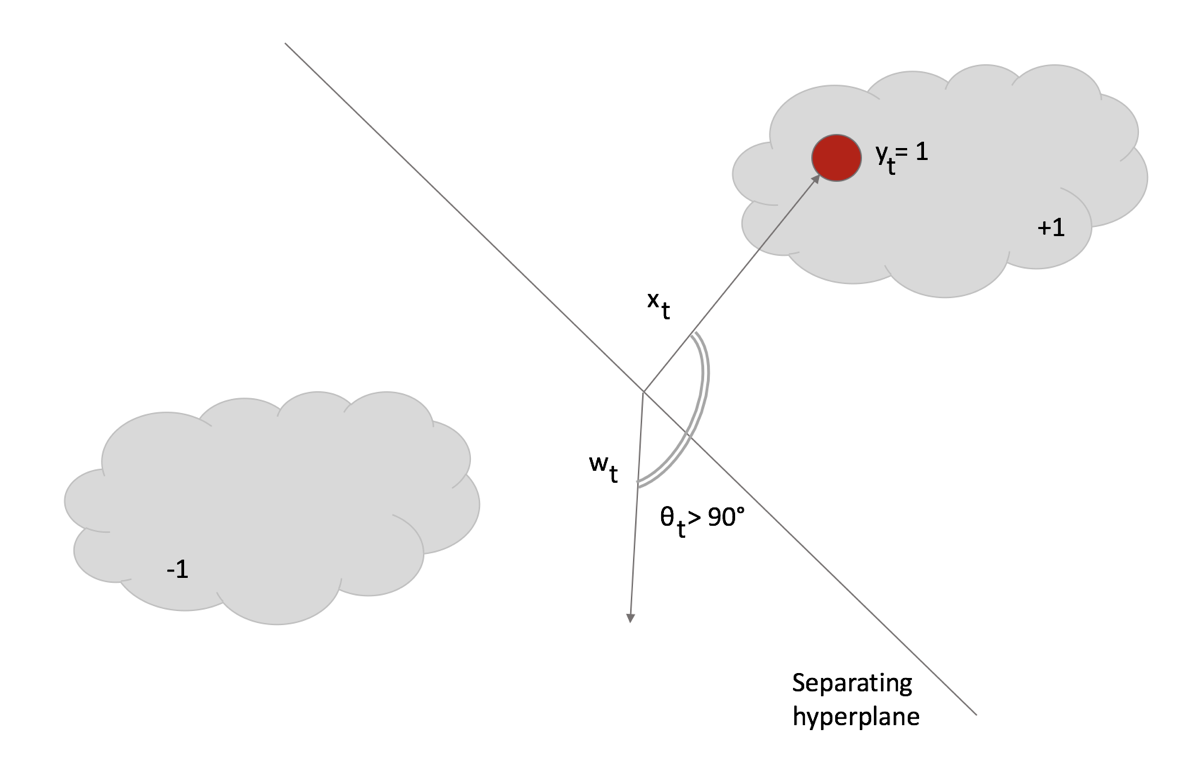
\includegraphics[scale=0.5]{Figure/PAII1.png}
    \caption{Iperpiano e vettore $w$, in fase passiva}
    \label{fig:PAII1}
\end{figure}
\FloatBarrier  

L'angolo $\theta> 90$, pertanto, il prodotto punto è negativo e il campione è classificato come $-1$, tuttavia la sua etichetta è $+1$. In questo caso, la regola di aggiornamento diventa molto aggressiva, perché cerca un nuovo $w$ che deve essere il più vicino possibile al precedente (altrimenti la conoscenza esistente viene immediatamente persa), ma deve soddisfare $L = 0$ (in altre parole, la classificazione deve essere corretta).

L'introduzione della variabile slack consente di avere margini \quotes{morbidi} (come in SVM) e un grado di tolleranza controllato dal parametro $C$. In particolare, la funzione di perdita deve essere $L \leq \xi$, consentendo un errore maggiore. Valori $C$ più alti producono una maggiore aggressività (con un conseguente rischio maggiore di destabilizzazione in presenza di rumore), mentre valori più bassi consentono un migliore adattamento. In effetti, questo tipo di algoritmi, quando si lavora online, deve far fronte alla presenza di campioni rumorosi (con etichette errate). È necessaria una buona robustezza, altrimenti cambiamenti troppo rapidi producono conseguenti tassi di classificazione errata più elevati.

Dopo aver risolto entrambe le condizioni di aggiornamento, otteniamo la regola di aggiornamento:

$$w_{t+1}=w_t+\frac{max(0,1-y_t(w^T\cdot x_t)}{\|x_t\|^2+\frac{1}{2C}}$$ 

Questa regola conferma le aspettative: il vettore di peso viene aggiornato con un fattore il cui segno è determinato da $y(t)$ e la cui grandezza è proporzionale all'errore. Nota che se non c'è classificazione errata il nominatore diventa $0$, quindi $w(t + 1) = w(t)$, mentre, in caso di classificazione errata, $w$ ruoterà verso $x(t)$ e si fermerà con una perdita $L \leq \xi$. Nella figura~\ref{fig:PAII2} successiva, l'effetto è stato contrassegnato per mostrare la rotazione, tuttavia è normalmente il più piccolo possibile.

\begin{figure}[h]
    \centering
    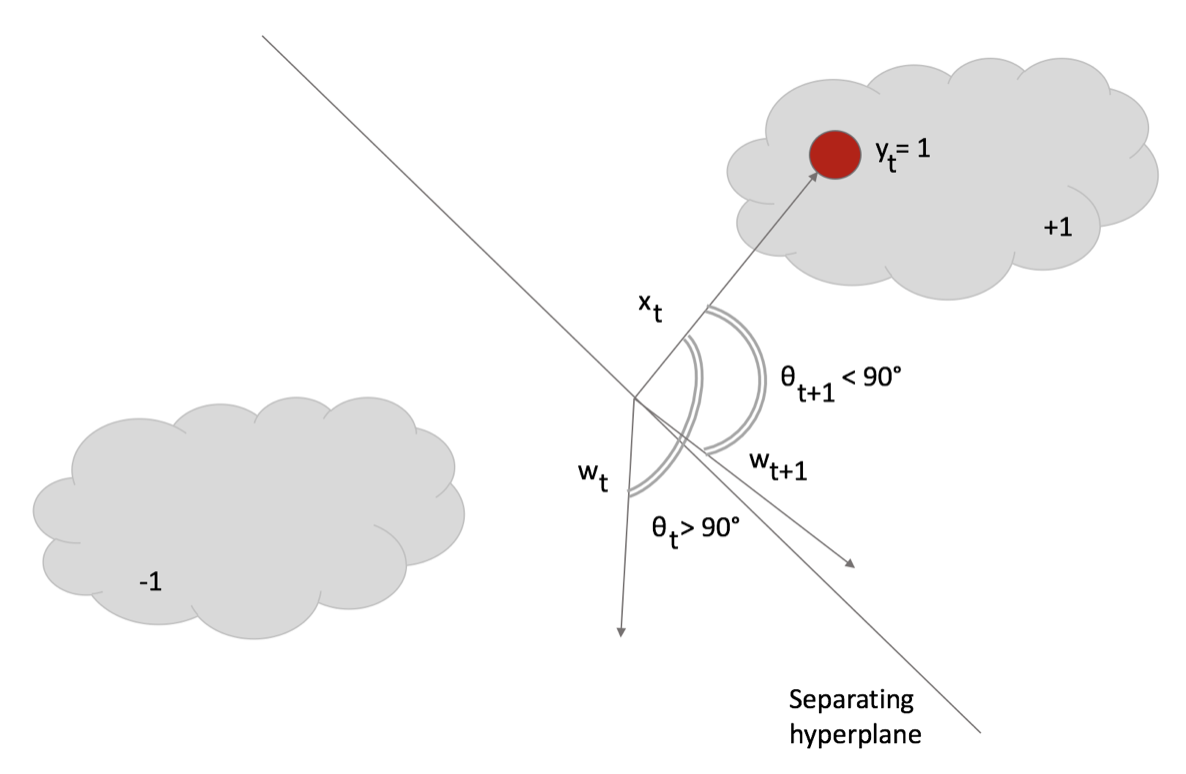
\includegraphics[scale=0.5]{Figure/PAII2.png}
    \caption{Rappresentazione dell'iperpiano e del vettore \textit{w} dopo l'update}
    \label{fig:PAII2}
\end{figure}
\FloatBarrier  


Dopo la rotazione, $\theta <90$ il prodotto punto diventa negativo, quindi il campione è correttamente classificato come $+1$.

L'idea è fornire all'utente un sistema già pre-addestrato che pian piano si adatti alle sue esigenze. Per questo scopo dobbiamo adottare una strategia di transfer-learning / multi-view learning\cite{transfer-learning} (vedi Figura~\ref{fig:approccisens}.

Si vuole addestrare il Customized Sensitiveness Classifier con una multi-view che include sia l'embed (single-view) sia la valutazione del sensitiveness classifier (single-view). Abbiamo utilizzato in particolare la tecnica \textit{early integration}. 

La \quotes{early integration} consiste nel concatenare le view singole cioè le caratteristiche associate all'embed e i risultati in probabilità ottenuti tramite il Topic-specific Sensitiveness Classifier; in questo modo ogni combinazione (concatenazione di due o più viste singole) rappresenta un campione nei set di dati. Quindi abbiamo ottenuto vettori da 514 elementi (512+2) dove i primi 512 elementi sono l'embed della frase e gli ultimi due sono la probabilità associata alla sensibilità negativa e la sensibilità positiva, rispettivamente.

\begin{figure}[h]
    \centering
    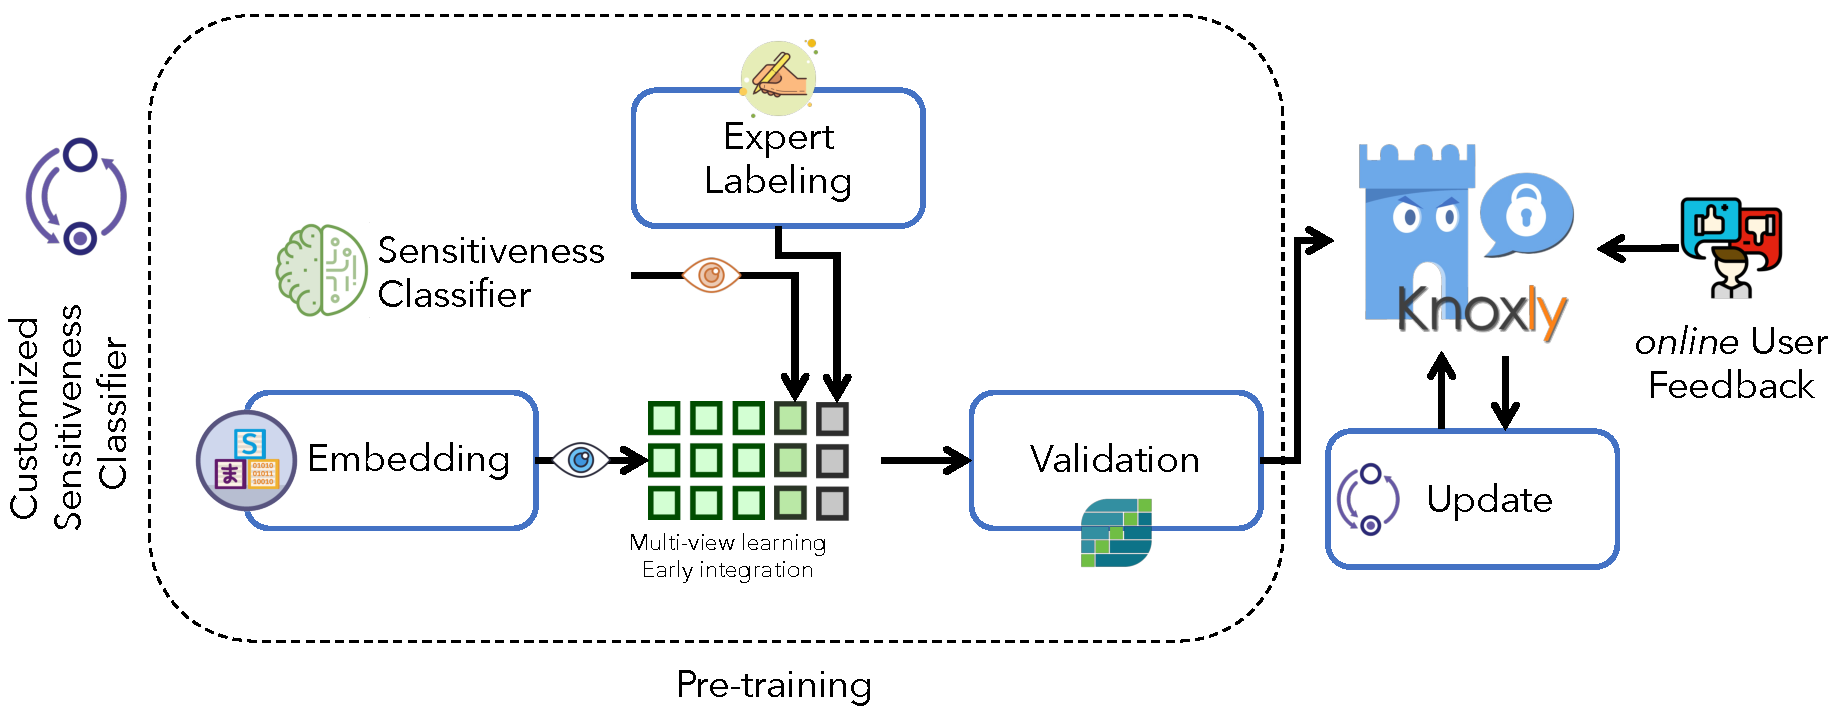
\includegraphics[width=15cm]{Figure/grafici/customized_cropped.pdf}
    \caption{schema riassuntivo del funzionamento del Customized Sensitiveness classifier}
    \label{fig:approccisensCustomized}
\end{figure}
\FloatBarrier

\subsection{Validation}
Abbiamo utilizzato i dataset {\tt ds200.csv} visti in Sezione~\ref{ssec:create_sens_ds} integrati con la valutazione del Topic-specific Sensitiveness Classifier di riferimento. Quindi il dataset {\tt ds200.csv} relativo al topic Health viene integrato con la valutazione di Health Sensitiveness classifier e così via per tutti gli altri.
I dataset sono stati suddivisi, con un approccio stratificato, in un 80\% per il training ed un 20\% per il testing utilizzando la funzione {\tt train\_test\_split} di scikit-learn per Python. Successivamente, il training set è stato oggetto di una 10-fold cross-validation con il metodo {\tt GridSearchCV} in cui abbiamo cercato di ottimizzare il parametro di aggressività $C$. Si osservi però che questo parametro è in realtà molto user-based, ragion per cui il miglior metodo per stimarlo potrebbe essere effettuando uno studio sugli utenti: è possibile che questi preferiscano un classificatore molto aggressivo o, al contrario, siano soddisfatti maggiormente con un apprendimento più lento e graduale. I valori di $C$ provati sono i seguenti: 0.001, 0.01, 0.1, 1, 10, 100. I risultati di questa fase possono essere visti in Tabella~\ref{tbl:testing_Customized}. Il miglior parametro è risultato essere per tutti i casi, $C=0.01$.

\subsection{Testing}
Una volta ottenuto il miglior parametro $C$ di aggressività per ciascun customized sensitiveness classifier procediamo con la fase di testing, in cui valutiamo le prestazioni del classificatore pre-addestrato su un set di dati ancora \quotes{intonso}, il test set, composto dal 20\% dei dati ds200.

\begin{table}[h!t]
\centering

\begin{tabular}{|c|c|c|c|c|}
\hline
\multicolumn{5}{|c|}{\textbf{Accuracy}} \\ \hline
\textbf{Politics} & \textbf{Health} & \textbf{Job} & \textbf{Travel} & \textbf{General} \\ \hline
0.835 & 0.98 & 0.95 & 0.975 & 0.965 \\ \hline
\end{tabular}
\caption{Tabella delle accuracy ottenute dal Customized Sensitiveness Classifier sui vari topic}
\label{tbl:testing_Customized}
\end{table}
\FloatBarrier
I risultati della fase di testing possono essere trovati in Tabella~\ref{tbl:testing_Customized}. Si nota come utilizzando questo approccio le performance del classificatore migliorino sensibilmente rispetto quelle ottenute in Sezione~\ref{sssec:multiclass}.


\chapter{Knoxly, un tool di privacy awareness}
Una volta implementato il core basato su Intelligenza Artificiale, in questo capitolo parliamo di come è stato sviluppato ed aggiornato il tool Knoxly.
 
Nella Sezione~\ref{sec:whoisKnoxly} sono stati spiegati il funzionamento, gli obiettivi e i limiti del progetto Knoxly, una estensione per Google Chrome volta a fornire privacy awareness agli utenti riguardo il contenuto dei messaggi che sono in procinto di pubblicare sul Web. Prima di questo lavoro Knoxly era in grado di segnalare all'utente la presenza di dati sensibili e/o personali presenti in un testo scritto in italiano o inglese basandosi su un analizzatore lessicale (quindi utilizzando una logica keyword-based). Ora Knoxly può contare su una analisi del testo migliore dato che adesso è dotato di tre moduli: (a) il \textit{Topic classifier} (Sez~\ref{sec:topicclass}) che è in grado di capire a quale fra cinque topic (politics, health, job, travel e general) appartiene un testo scritto in una tra 16 lingue (vedi Sezione~\ref{sec:use}), (b) il \textit{Sensitivity classifier} (Sezione~\ref{sec:sensclass}) che è in grado di comprendere quanto un testo sia sensibile o meno (sempre in 16 lingue) e (c) il \textit{Customized sensitivity classifier} (Sezione~\ref{sec:pres_sens_class}) che è in grado apprendere le preferenze degli utenti in fatto di privacy e regolare le segnalazioni di Knoxly di conseguenza.

Più nello specifico, in questo capitolo si mostra il flusso di lavoro di Knoxly (Sezione~\ref{sec:workflow}), il client-side con la User Interface (UI) (Sezione~\ref{sec:frontend}) e il server-side (Sezione~\ref{sec:backend}).

\section{Workflow}
\label{sec:workflow}
In questa sezione si descrivono i vari step che affronta un testo scritto in linguaggio naturale analizzato da Knoxly. In figura~\ref{fig:workflow} è presente una illustrazione del flusso di lavoro del tool e di come le varie componenti interagiscono tra loro.

\begin{figure}[h]
    \centering
    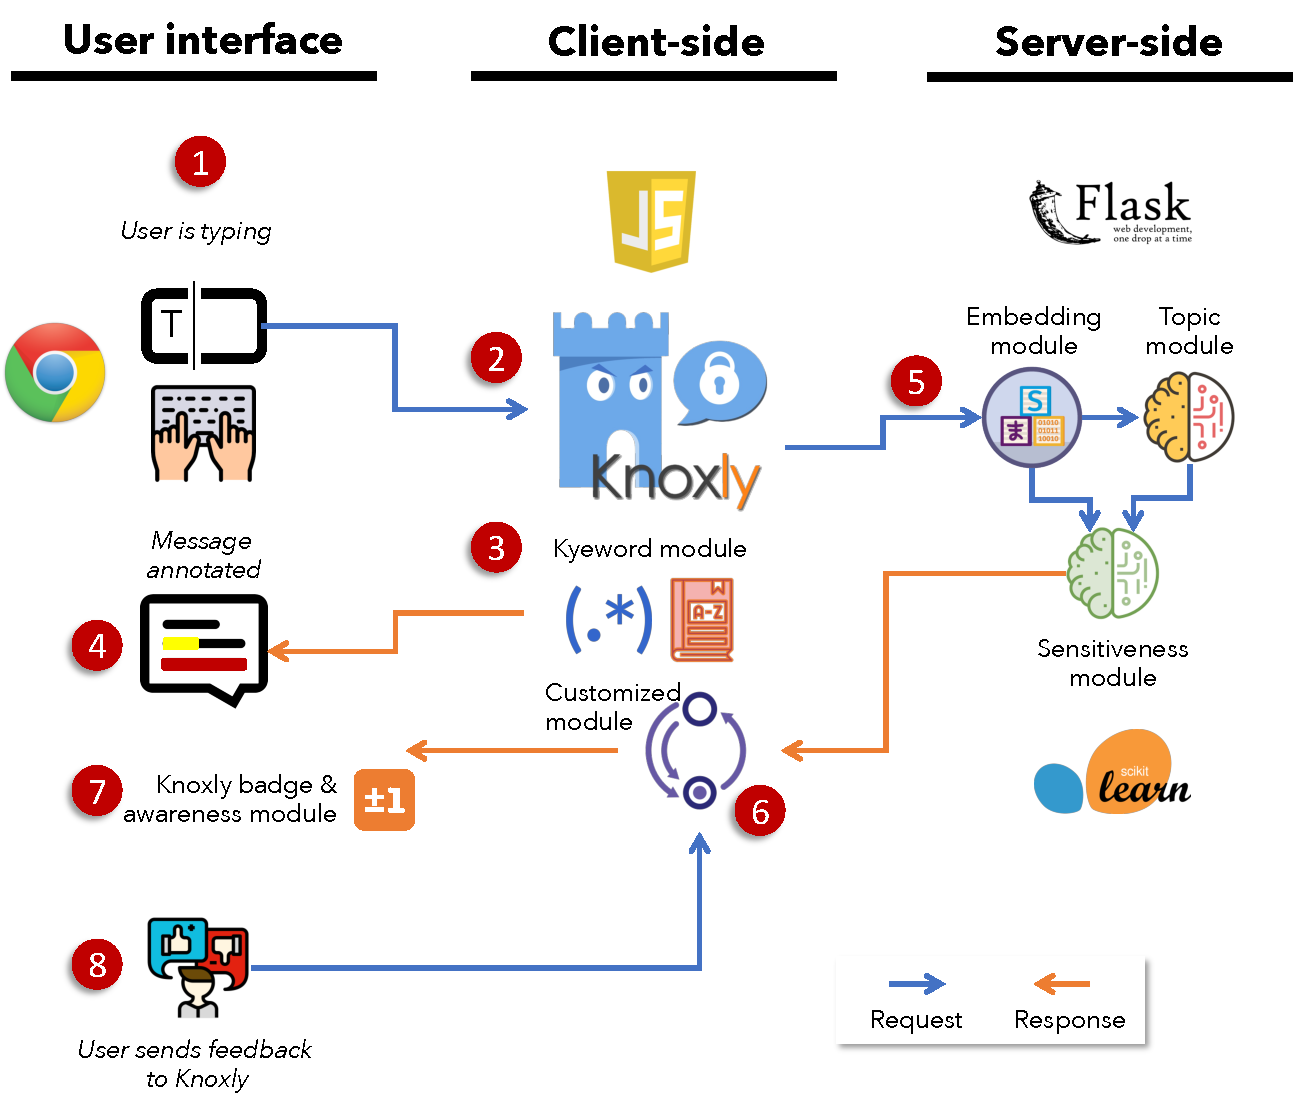
\includegraphics[width=15cm]{Figure/workflow.pdf}
    \caption{schema riassuntivo del workflow di Knoxly}
    \label{fig:workflow}
\end{figure}
\FloatBarrier
L'interazione che un utente ha con Knoxly avviene nel seguente modo:
\begin{enumerate}
    \item L'utente digita un testo $t$;
    \item Il testo $t$ viene inviato al plug-in Knoxly;
    \item $t$ viene innanzitutto analizzato con il \textit{Keyword module} utilizzando espressioni regolari e dizionari (codificati in Knoxly);
    \item Le keyword in $t$ che hanno una corrispondenza con le espressioni regolari o con i dizionari vengono evidenziate con l'ausilio di un tag {\tt <span>} a cui è associata una opportuna classe {\tt .css} (\textit{giallo} per i quasi identifier~\cite{} e dati sensibili, \textit{rosso} per i dati personali). Si fornisce inoltre la possibilità di anonimizzare le keyword segnalate utilizzando la k-anonimity~\cite{} (qui termina l' analisi lessicale);
    \item Knoxly invia $t$ al server Flask\footnote{https://flask.palletsprojects.com/en/1.1.x/} il quale effettua l'embedding della frase tramite l'embedding module (basato su multilingual Universal Sentence Encoder), dopidichè invia l'embed al \textit{Topic module} ed al \textit{Sensitiveness module}. Il Topic module, basato sul Topic classifier, stabilisce a quale topic appartiene $t$. In base a questo si richiama l'opportuno \textit{Sensitiveness Classifier} nel \textit{Sensitiveness module}. Quest'ultimo restituisce un vettore di due elementi (sensibilità negativa e sensibilità positiva), percentuale delle classi,  il quale, insieme all'embed verranno restituiti al client-side.
    \item Il server invia al client un vettore di 514 elementi ovvero l'embed (512 elementi) con accodatio il vettore della probabilità delle classi (2 elementi) restituito dal \textit{Sensitiveness module}. Questa risposta viene elaborata dal \textit{Customized sensitiveness module}, il quale (a) la smista al \textit{Customized Sensitiveness classifier} adatto a quel topic, (b) valuta se il contenuto risulta sensibile secondo la percezione della privacy che ha l'utente.
    \item Se il \textit{Customized Sensitiveness classifier} classifica il contenuto restituitogli dal server come sensibile, cioè un contenuto che rappresenta una minaccia alla privacy dell'utente, allora lo segnala all'utente incrementando un contatore numerico posto in un badge dell'icona di Knoxly in Google Chrome, oltre ad aggiungerlo in una list box - progettata per fornire awareness - consultabile aprendo il popup del tool.
    \item L'utente ha la possibilità di cliccare su di un bottone \quotes{feedback} indicando a Knoxly di evitare di segnalare (come sensibili) in futuro quel tipo di testi. Tale operazione aggiorna i pesi del \textit{Customized Sensitiveness Classifier} di riferimento per i testi appartenenti a quel topic.
\end{enumerate}

\section{Client-side}
\label{sec:frontend}
In questa sezione si dettagliano le caratteristiche del lato client di Knoxly.

\subsection{Euristica di input}
\label{ssec:euristicInput}
Uno dei problemi affrontati in fase di sviluppo è comprendere quando è più opportuno chiamare i moduli basati su intelligenza artificiale di Knoxly. È evidente che l'utilizzo smisurato di moduli del backend risulterebbe in un appesantimento del servizio, rendendolo lento, fastidioso e inutilizzabile. Inoltre ciò comporterebbe l'analisi di testi che non rappresentano vere e proprie frasi, cioè composte da almeno \textit{soggetto}, \textit{predicato} e \textit{complemento}, o comunque che includono un numero tale di parole da poterne comprendere la semantica. Quindi, in altri termini, la domanda è\textit{ "quando è il momento adatto per inviare una frase al server e quando invece bisogna solo affidarsi al Keyword module?"}.

Per rispondere a questo quesito bisogna definire una \textit{euristica di input} che deve garantire l'invio di frasi verso il server di Knoxly senza rischiare di creare un collo di bottiglia. 

L'euristica di input è stata definita come segue: sia $txt$ il vettore contenente i caratteri che l'utente ha digitato, $n$ la lunghezza del vettore $txt$, $txt[last]$ l'ultimo carattere presente in $txt$ e $T = \{".", ";", "!", "?"\}$ l'insieme dei caratteri che vengono posti alla fine di una frase scritta in linguaggio naturale, allora
$$ n>=5 \And txt[last] = x \in T \implies \text{invia txt al server}$$.
L'invio della frase al server avviene tramite una chiamata {\tt AJAX} verso l'endpoint del server di Knoxly. Quando arriva la risposta dal server viene chiamato il \textit{Customized Sensitiveness module} per valutare se il testo risulta sensibile anche sulla base della percezione di privacy che ha l'utente.

\subsection{User Interface per fornire privacy awareness}
\label{ssec:ui}


La User Interface (UI) di Knoxly è stata progettata ed implementata per fornire privacy awareness in modo semplice ed intuitivo. Come anticipato in Sezione~\ref{sec:whoisKnoxly} Knoxly evidenzia contenuti sensibili e/o personali presenti in un testo scritto in italiano o in inglese tramite l'utilizzo di espressioni regolari e dizionari. Utilizziamo il \textit{giallo} per i quasi identifier~\cite{} e dati sensibili, il \textit{rosso} per i dati personali. 

Cliccando sull'icona posta accanto alla barra dell'indirizzo su Google Chrome, viene visualizzato il popup di Knoxly. Accanto all'icona è possibile inoltre visualizzare un badge che riporta un contatore numerico (vedi Figura~\ref{}). Tale contatore è utilizzato per segnalare all'utente il numero di frasi scritte classificate come minacce per la sua privacy, cioè sensibili. 

\begin{figure}[h]
    \centering
    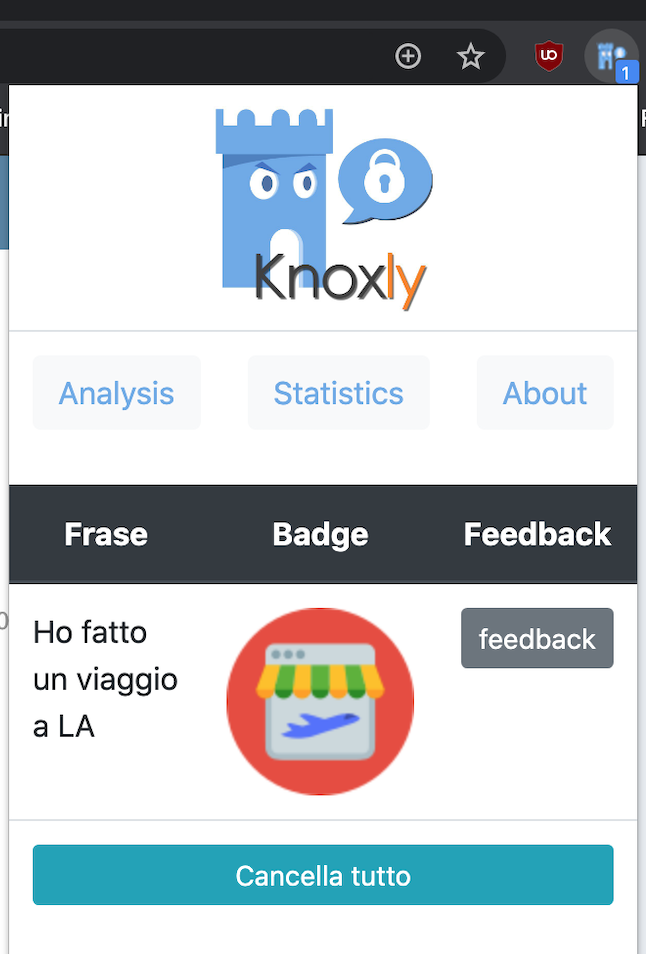
\includegraphics[scale=0.7]{Figure/ui/UI-Knoxly.png}
    \caption{User Interface di Knoxly}
    \label{fig:uiKnoxly}
\end{figure}
\FloatBarrier

In Figura~\ref{fig:uiKnoxly} viene mostrata la landing page una volta aperto il popup di Knoxly. La UI del popup è composta principalmente da tre sezioni/pagine:
\begin{itemize}
    \item \textbf{Analysis}: pagina dedicata alle segnalazioni del tool. La pagina fa anche da landing page;
    \item \textbf{Statistics}: pagina dedicata alle misurazioni, utili a rendere l'utente consapevole di ciò che scrive e quanto;
    \item \textbf{About}: pagina dedicata ad istruzioni sull'utilizzo di Knoxly.
\end{itemize}

\textbf{Analysis} è composta da una tabella con 3 colonne. Mostra le frasi che Knoxly reputa sensibili, indicando una icona facente riferimento al topic a cui appartiene la frase che può avere due colori: \textit{giallo} nel caso in cui la frase risulti sensibile (sensibilità positiva compresa fra $0.36$ e $0.68$) o \textit{rosso} nel caso in cui la frase abbia una sensibilità positiva maggiore o uguale a $0.68$. Inoltre viene mostrato anche il bottone \textbf{feedback} che consente all'utente di inviare un feedback a Knoxly per far si che il tool non segnali più come sensibili frasi simili a quella per cui si sta inviando il feedback.

Le icone scelte per fornire consapevolezza sono mostrate in Figura~\ref{}. Sono stati utilizzati i colori \textit{rosso} e \textit{giallo} 

La sezione \textbf{Statistics} (vedi Figura~\ref{fig:statKnoxly} è dedicata alle misurazioni: l'utente può visualizzare un grafico a barre che riporta il numero di occorrenze di frasi sensibili che lui ha divulgato in rete nei vari topic, politica, salute, viaggi, lavoro e general. Al di sotto del grafico a barre l'utente può visualizzare l'\textbf{overall score} della sensibilità dei contenuti che divulga in rete. L'overall score $s$ viene calcolato con il seguente algoritmo 

L'overall score non è altro che il calcolo online della media degli score di sensibilità ottenuti per ciascuna delle frasi che ha divulgato, con riferimento alle sole frasi classificate sensibili. $s \in [0..1]$ e viene rappresentato come un cerchio che si colora di rosso se l'overall score supera 0.68 altrimenti è mostrato in giallo. 
\begin{figure}[h]
    \centering
    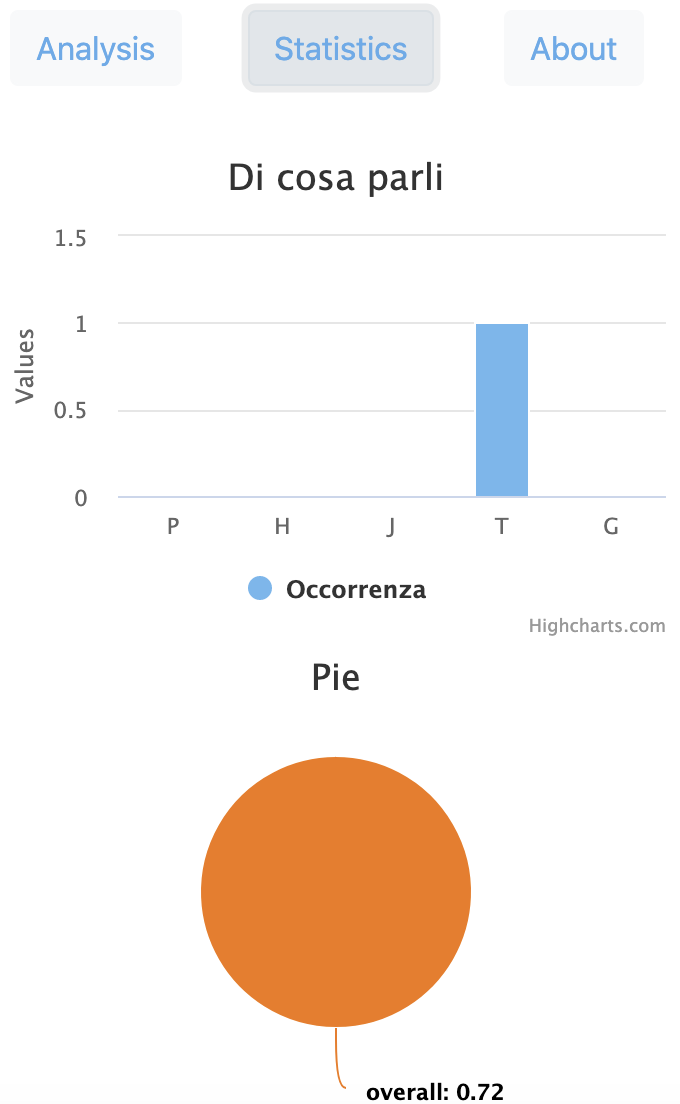
\includegraphics[scale=0.7]{Figure/ui/statistics.png}
    \caption{sezione statistics di Knoxly}
    \label{fig:statKnoxly}
\end{figure}
\FloatBarrier

Infine nella sezione \textbf{About}(figura \ref{fig:about}) vengono riportate le informazioni riguardanti i bollini che fanno riferimento ai topic di Knoxly.
\begin{figure}[h]
    \centering
    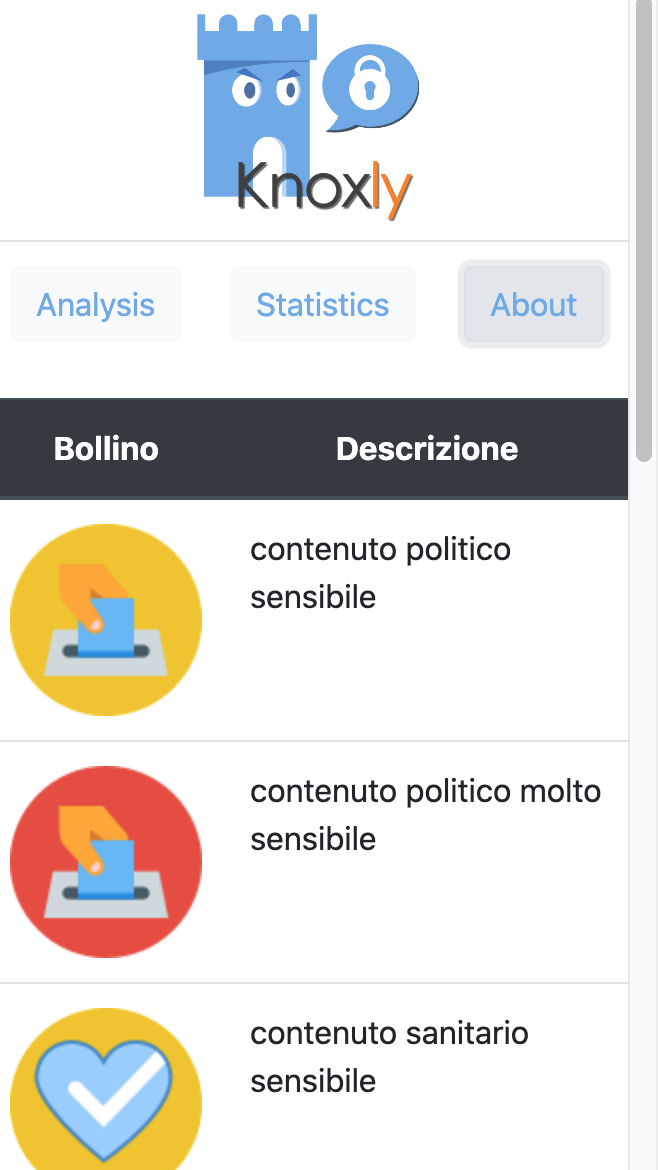
\includegraphics[scale=0.7]{Figure/ui/about.png}
    \caption{sezione about di Knoxly}
    \label{fig:about}
\end{figure}
\FloatBarrier
La UI di Knoxly è stata realizzata utilizzando Bootstrap\footnote{https://getbootstrap.com/}, e Highcharts\footnote{https://www.highcharts.com/} per i grafici.

\section{Server-side}
\label{sec:backend}
Il lato server di Knoxly è molto semplice esso è stato realizzato in Flask\footnote{https://flask.palletsprojects.com/en/1.1.x/} ed è composto da un unico end point, questo riceve la frase del client, effettua l'embed utilizzando USE, chiama il Topic classifier e in base al topic individuato chiama il Sensitiveness classifier di competenza, dopodichè invia l'embed con accodato il vettore contenente la sensibilità negativa e positiva al client affichè questo possa valutare se la frase risulta sensibile anche per la percezione di privacy che ha l'utente.

\chapter{Evaluation}
In questo capitolo verrà spiegata come è stata effettuata la valutazione delle perfomance del plug-in. Le perfomance sono state valutate in termini di \textbf{efficacia}, ovvero, quanto siano accurate le previsioni effettuate, ed \textbf{efficienza}, ovvero, quanto tempo, spazio e CPU utilizza il plug-in.   

\section{Metodologia utilizzata}
\label{sec:metodologiaevaluation}
L'analisi qualitativa e qualitativa è state effettuata cercando di calare quanto più possibile il plug-in in un contesto reale. Per fare cioè esso doveva effettuare le sue predizioni su degli input che non aveva mai visto. A tal fine è stato scelto da \href{https://www.kaggle.com/}{kaggle.com} il dataset {\tt Sentiment140 dataset with 1.6 million tweets }\cite{sentiment140} dalla quale sono state selezionate 500 entry con una funzione {\tt random}.

Per inviare le 500 entry al backend di Knoxly è stato realizzato un bot con \href{https://selenium-python.readthedocs.io/}{Selenium with Python}. Esso interagisce con una pagina web e inviava la frase al backend secondo i criteri definiti  dall'euristica per l'invio della frase(Sez. \ref{sec:frontend}).

Durante l'invio delle frasi il backend registra (i) tempo (in secondi), (ii) RAM utilizzata (in Megabytes) e (iii) CPU utilizzata (in percentuale dove ogni thread utilizzato a pieno corrisponde al 100\%\footnote{Una macchina con 2 core, 4 thread può avere un consumo di CPU massimo del 400\%.}), mentre, il backend misura (i) RAM (in Megabytes) e (ii) CPU utilizzata (in percentuale) con e senza l'utilizzo di Knoxly.

Infine i risultati vengono raccolti e mostrati sotto forma di grafici e matrici.

\begin{figure}[h!t]
    \centering
    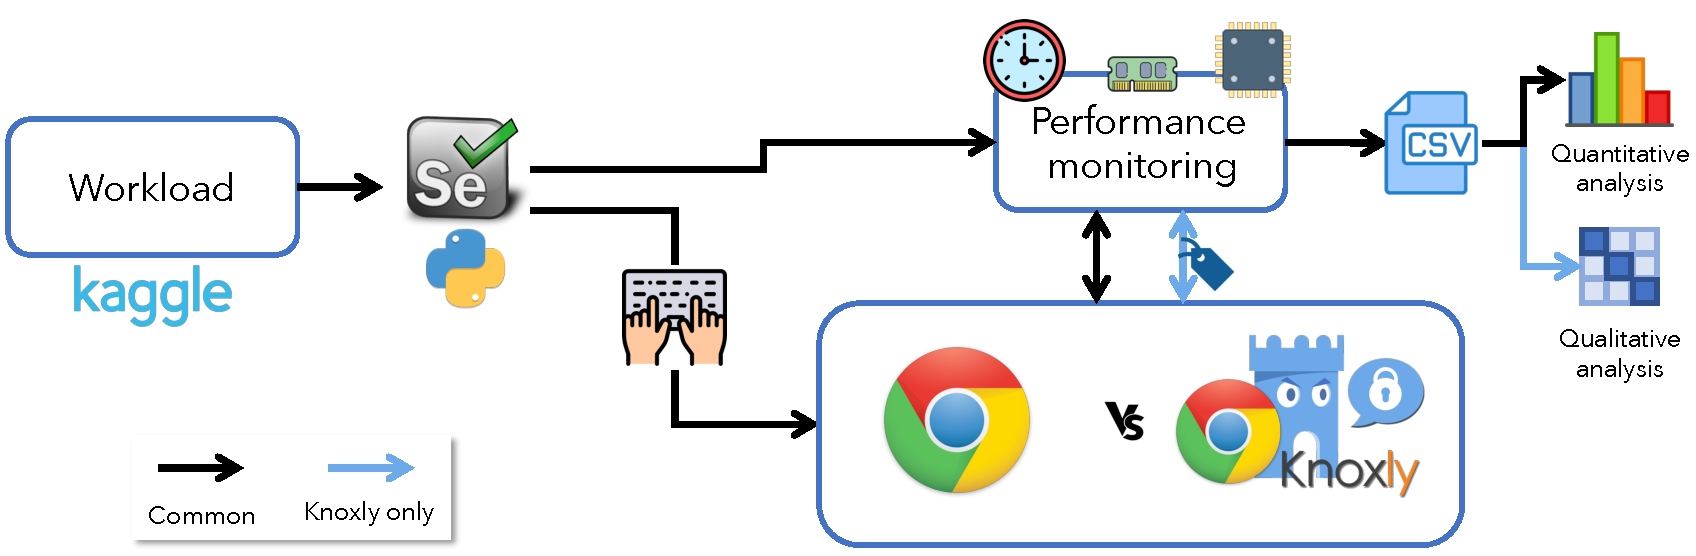
\includegraphics[width=15cm]{Figure/grafici/evaluation_cropped.pdf}
    \caption{Workflow della metodologia utilizzata}
    \label{fig:methodeval}
\end{figure}
\FloatBarrier

\section{Qualitative Analysis}
\label{sec:quantitative}
Una analisi qualitativa è stata effettuata al fine di valutare le performance sia del backend che del frontend in termini tempi di esecuzione, \%CPU utilizzata e RAM utilizzata.
\subsection{Server-side}
\label{sec:quantbackend}
Delle frasi che sono state inviate al backend vengono prese le seguenti misure:
\begin{itemize}
    \item \textbf{Tempo}: per tempo si intende solo il tempo in secondi impiegato dal server per smaltire la richiesta che gli è arrivata. Questa misura non tiene conto della latenza fra client e server
    \item \textbf{\% Utilizzo CPU}: percentuale di CPU utilizzata dal server per smaltire una richiesta 
    \item \textbf{RAM allocata}: Mb di RAM utilizzati dal server per smaltire una richiesta
\end{itemize}

\paragraph{Tempo}

\begin{figure}[h!t]
    \centering
    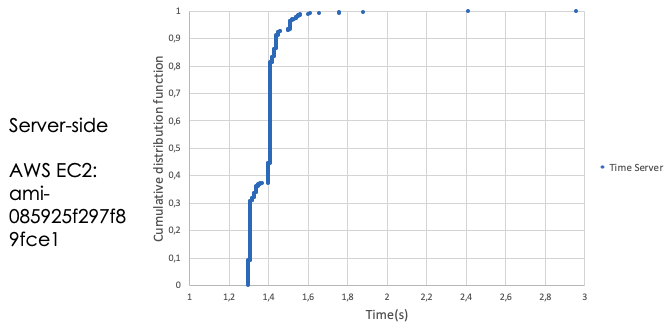
\includegraphics[width=15cm]{Figure/quantitativa/timeSrv.png}
    \caption{grafico dei secondi impiegati dal server per smaltire una richiesta}
    \label{fig:srvTime}
\end{figure}
\FloatBarrier

Si nota che il server in genere impiega dagli 1.3 agli 1.6 secondi per smaltire una richiesta, raramente impiega più di due secondi e che non impiega mai 3 secondi o più.

\paragraph{\% Utilizzo CPU}
\begin{figure}[h!t]
    \centering
    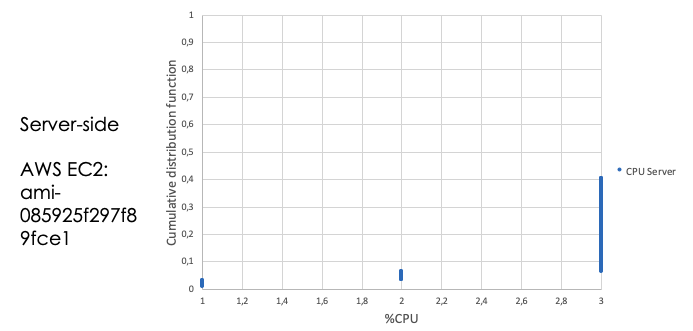
\includegraphics[width=15cm]{Figure/quantitativa/CPU-srv.png}
    \caption{grafico della percentuale di CPU impiegata per smaltire le richieste}
    \label{fig:srvCPU}
\end{figure}
\FloatBarrier

Si nota che il server generalmente utilizza il 3\% della sua CPU per smaltire le richieste  e che solo nelle fasi iniziali arriva ad utilizzare l'1 o il 2 percento della CPU.

\paragraph{RAM allocata}
\begin{figure}[h!t]
    \centering
    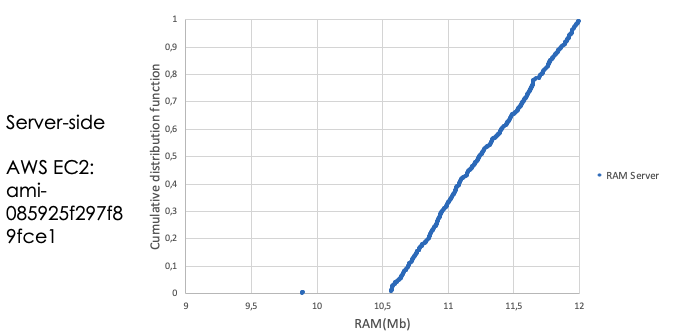
\includegraphics[width=15cm]{Figure/quantitativa/quant_RAM-srv.png}
    \caption{grafico dei Mb di RAM impiegati per smaltire le richieste}
    \label{fig:srvRAM}
\end{figure}
\FloatBarrier

Si nota che il consumo di RAM, lato backend, è compreso fra i 10.5 e i 12 Mb di RAM

\subsection{Client-side}
\label{sec:quantClient}
Delle frasi che sono state inviate al frontend vengono prese le seguenti misure:
\begin{itemize}
    \item \textbf{\% Utilizzo CPU Chrome e \%Utilizzo Knoxly}: percentuale di CPU utilizzata solo da Chrome durante l'invio delle frasi e percentuale di CPU utilizzata sola da Knoxly. 
    \item \textbf{RAM allocata da Chrome e RAM allocata da Knoxly}: Mb di RAM utilizzati da solo Chrome durante l'invio delle frasi e Mb di RAM utilizzati solo da Knoxly.
\end{itemize}

\paragraph{\% Utilizzo CPU Chrome e \%Utilizzo Knoxly}
\begin{figure}[h!t]
    \centering
    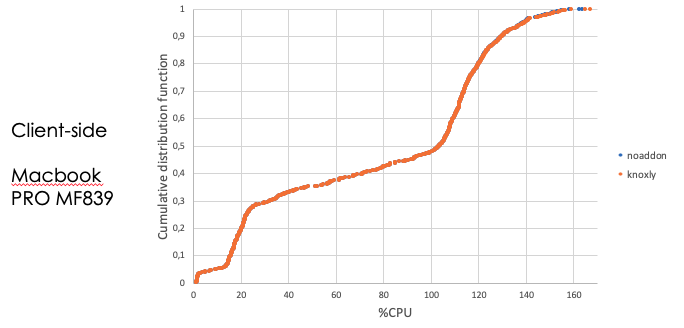
\includegraphics[width=15cm]{Figure/quantitativa/CPU-client.png}
    \caption{grafico della percentuale di CPU impiegata da Knoxly(punti arancioni) e da Chrome(punti blu)}
    \label{fig:clientCPU}
\end{figure}
\FloatBarrier

Dal grafico si evince che l'andamento dell'utilizzo delle percentuale di CPU solo di Knoxly è sovrapposto all'andamento dell'utilizzo della CPU solo da parte di Chrome. Quindi possiamo dire che Knoxly e Chrome utilizzano la stessa percentuale di RAM durante l'invio delle frasi e che Knoxly e Chrome al massimo arrivano ad utilizzare il 160\% della CPU,ovvero,poco più di un core e mezzo.

\paragraph{RAM allocata da Chrome e RAM allocata da Knoxly}
\begin{figure}[h!t]
    \centering
    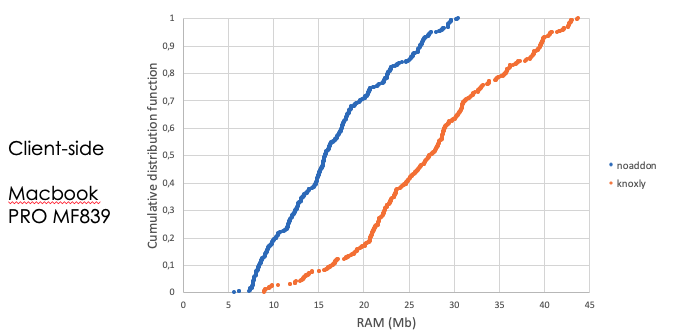
\includegraphics[width=15cm]{Figure/quantitativa/RAM-client.png}
    \caption{grafico dei Mb di RAM impiegati da Knoxly(punti arancioni) e da Chrome(punti blu)}
    \label{fig:clientRAM}
\end{figure}
\FloatBarrier
Dal grafico si evince che inizialmente Knoxly occupa più RAM rispetto a Chrome e questo può essere dovuto al fatto che il plug-in inizialmente deve caricare in memoria tutti i dizionari e le regexp di cui necessita per effettuare l'analisi lessicale e l'evidenziazione di un testo sensibile.



\section{Qualitative Analysis}
\label{sec:qualitative}
L'analisi qualitative è stata effettuata per valutare quanto i classificatori realizzati siano in grado di effettuare delle predizioni corrette. Per tenere traccia delle predizioni effettuate dai classificatori su un file {\tt csv} sono state salvate le frasi processate, il topic alla quale appartengono secondo la predizione effettuata dal {\tt Topic classifier} e la sensibilità della frase secondo la predizione effettuata dal {\\ Sensitiveness classifier}.

\subsection{Topic classifier}
\label{sec:qualTopic}

\begin{figure}[h!t]
    \centering
    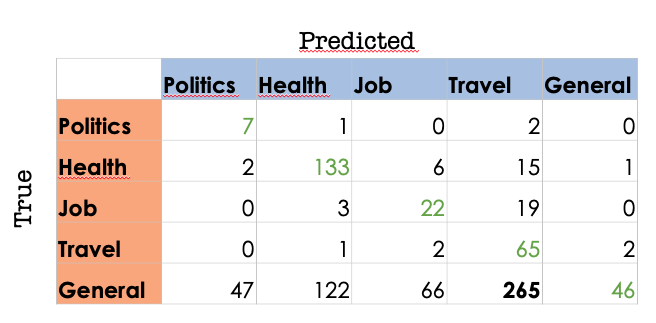
\includegraphics[width=15cm]{Figure/qualitativa/qual_topic.png}
    \caption{matrice di confusione del Topic classifier}
    \label{fig:confMtrTopicClass}
\end{figure}
\FloatBarrier

In Figura~\ref{fig:confMtrTopicClass} è mostrata la matrice di confusione ottenuta nella fase di evaluation. Si può notare che il Topic Classifier effettua il maggior numero di predizioni corrette sul topic health, mentre,il Topic classfier sbaglia spesso nel classificare una frase appartenente al topic general come una frase appartenente al topic travel. Questo a causa (a) del dataset utilizzato per l'addestramento che nel caso del topic \textit{travel} è fatto di tweet postati su Twitter (più simili morfo-sintatticamente a quelli utilizzati in questo test), nell'altro caso è una descrizione più articolata di una trama di un film (alquanto dissimile rispetto i testi utilizzati in questo test), (b) tweet molto brevi. Questo secondo problema è infatti motivo di molti errori.

Per questo motivo, abbiamo calcolato la media della lunghezza delle frasi contenute nel nostro workload ed abbiamo usato questo valore come soglia minima per considerare i tweet in una analisi che coinvolgesse solo quelle più lunghe. In particolare la media è 70 caratteri, per cui in questa seconda analisi consideriamo solo i tweet che contengono più di 70 caratteri.

\begin{figure}[h!t]
    \centering
    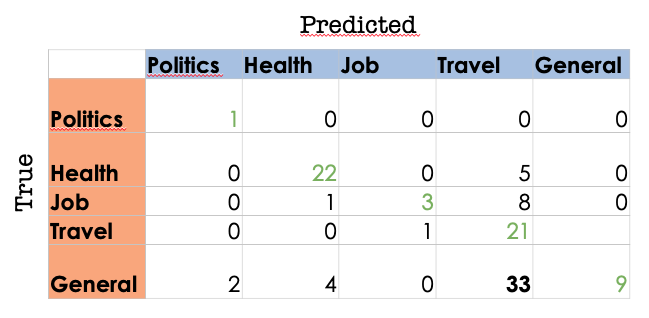
\includegraphics[width=15cm]{Figure/qualitativa/qual70char.png}
    \caption{matrice di confusione del Topic classifier dei soli testi maggiori di 70 caratteri}
    \label{fig:confMtrTopicClassGT70}
\end{figure}
\FloatBarrier

In Figura~\ref{fig:confMtrTopicClassGT70} è mostrata la matrice di confusione per il Topic classifier quando consideriamo solo tweet con lunghezza $l > 70$. L'ipotesi precedentemente formulata risulta vera. Infatti considerando solo frasi più lunghe il risultato migliora. Anche in questo caso si può notare che il topic con il numero più alto di veri positivi è health, seguito da travel. Il topic dove incontriamo maggiori errori di classificazione resta \textit{general}. Il Topic classifier anche su input più lunghi continua a sbagliare classificando come \textit{travel} frasi appartenenti a \textit{general}.

\subsection{Sensitiveness classifier}
\label{sec:qualSens}
Il secondo modulo di Knoxly di cui si vuole valutare l'efficacia è il Sensitiveness Classifier. Si osserva se una frase classificata come sensibile, quindi avendo con uno score di $probabilitaPositiva \geq 0.50$, è realmente sensibile in accordo alla euristica sulla sensibilità definita in Sez.~\ref{sssec:sens_labeling}. 

\begin{figure}[h!t]
    \centering
    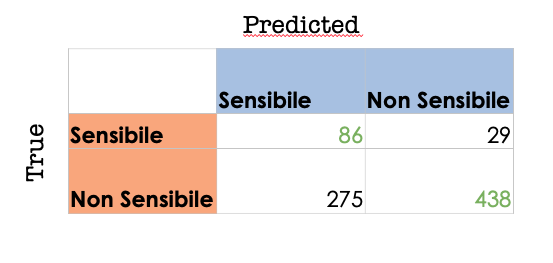
\includegraphics[width=15cm]{Figure/qualitativa/qualSens.png}
    \caption{matrice di confusione del sensitiveness classifier}
    \label{fig:sensitivenessevaluation}
\end{figure}
\FloatBarrier

In figura~\ref{fig:sensitivenessevaluation} è riportato il risultato di questa analisi di efficacia. Si può notare che il numero di falsi positivi è maggiore del numero dei falsi negativi. Da ciò si evince che il Sensitiveness Classifier individua e segnala più contenuti sensibili rispetto a quanti ne dovrebbe segnalare. Questo è un falso problema dal momento che si preferisce avere un classificatore che segnali un non sensibile come sensibile e non viceversa altrimenti dei dati sensibili e/o personali rischierebbero di essere divulgati in rete. Resta comunque il fatto che l'utente può addestrare il plug-in sul suo livello di privacy in base ai feedback che invia, facendo così diminuire il numero di segnalazioni.

\subsection{Customized Sensitiveness classifier}
\label{sec:qualCusto}
Per testare il modulo di Customized Sensitiveness Classifier abbiamo automatizzato con Selenium la digitazione di testo in linguaggio naturale e l'invio feedback al customized sensitiveness classifier lato client. L'idea è stata quella di preparare un dataset di testi che risultano essere sensibili e farli classificare al customized sensitiveness classifier. Per ciascun testo, vogliamo inviare a Knoxly un feedback negativo e ripetere la classificazione dell'intero dataset. Ci aspettiamo che se il customized sensitiveness classifier apprende in modo corretto dall'utente, allora l'accuratezza risultante dalla classificazione diminuisce con l'aumentare dei feedback.

Per questo esperimento abbiamo utilizzato un dataset minimale, composto da 10 elementi sensibili per ciascun topic (health, politics, travel, general, job). Abbiamo incrementato la taglia di questo dataset del 200\% popolandolo con frasi di significato simile ma scritte in altre lingue (italiano in particolare) o utilizzando sinonimi. Per il primo caso abbiamo utilizzato deepl\footnote{\url{https://www.deepl.com/translator}}, un famoso..., nel secondo invece, Reverso\footnote{\url{https://synonyms.reverso.net/synonym/}}, un servizio online che aiuta gli utenti nelle traduzioni domain-specific e nella ricerca di sinonimi. In tabella~\ref{tab:datasetcustomized} ne è riportato un esempio per il topic travel.


\begin{table}[h!t]
\centering
\begin{tabular}{l|p{9cm}}
\toprule
\textbf{Frase originale} & united Not sure what you are talking about She is going on nonstop flights SNA to SFO and then SFO to EWR \\
\midrule
\textit{Reverso} & united Not sure what you are speaking about She is riding on nonstop flights SNA to SFO and then SFO to EWR \\ 
\midrule
\textit{deepl} & united Non so di cosa stai parlando Lei sta andando su voli nonstop da SNA a SFO e poi SFO a EWR \\
\bottomrule
\end{tabular}
\caption{Esempio di data-augmentation per il dataset Travel nell'esperimento di efficacia per il Customized Sensitiveness Classifier. \textit{Reverso}: refactoring della frase utilizzando il famoso servizio online, \textit{deepl}: traduzione della frase dall'inglese all'italiano.}
\label{tab:datasetcustomized}
\end{table}
\FloatBarrier

Il risultato dell'esperimento è incoraggiante in quanto tutti i classificatori diminuiscono le loro performance via via che l'utente (bot selenium in questo caso) invia feedback negativi. In particolare in Figura~\ref{fig:plot_acc-health} e Figura~\ref{fig:plot_acc-travel} si mostrano i risultati ottenuti per Health e Travel, rispettivamente. Notiamo che, nel caso di Health, bastano pochi feedback per migliorare la conoscenza del classificatore e far adattare le sue segnalazioni alla percezione utente di privacy. Nel caso di Travel invece, l'utente ha bisogno di inviare più feedback prima che il classificatore comprenda le sue esigenze, in particolare ha bisogno di circa 10-12 feedback prima di apprendere bene "cosa si aspetta l'utente".

\begin{figure}[h!t]
    \centering
    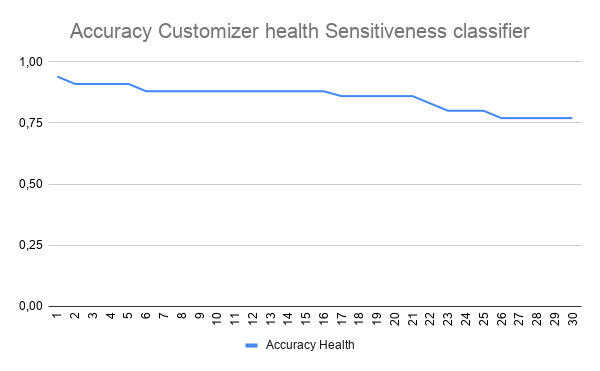
\includegraphics[width=15cm]{Figure/qualitativa/Custom_health-Sens.png}
    \caption{Scatter plot della accuracy del Customized Sensitiveness classifier sul topic health}
    \label{fig:plot_acc-health}
\end{figure}
\FloatBarrier

\begin{figure}[h!t]
    \centering
    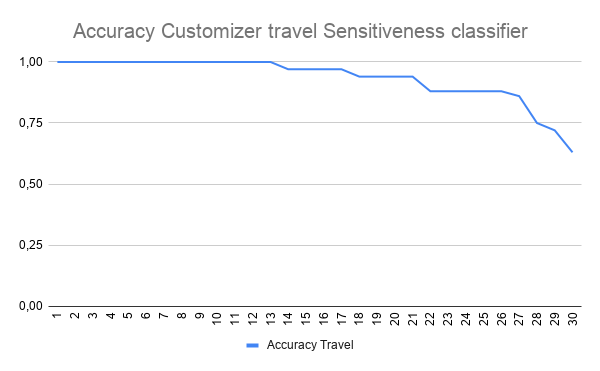
\includegraphics[width=15cm]{Figure/qualitativa/Customizer_travel-Sens.png}
    \caption{Scatter plot della accuracy del Customized Sensitiveness classifier sul topic travel}
    \label{fig:plot_acc-travel}
\end{figure}
\FloatBarrier



\chapter{Conclusioni e sviluppi futuri}
\label{ch:cap7}
Da quando 10-15 anni fa gli Online Social Network hanno iniziato a far parte delle vite di ciascun individuo, molti più dati vengono condivisi in rete. Tantissime persone divulgano spesso inconsapevolmente dati personali e sensibili che minano la privacy propria e degli altri. Nasce quindi l'esigenza di proteggere le persone non solo, come già avviene~\cite{}, da tracker in rete, ma anche da loro stessi, muovendosi verso un concetto di privacy un po' diverso, esteso, che può essere riassunto come segue: \textit{ \quotes{privacy as having the ability to control the dissemination of sensitive information}}.

Per questo motivo sorge la necessità di avere strumenti adatti a fornire consapevolezza agli utenti, avvertirli prima della divulgazione di informazioni sensibili o personali, fornendo quindi un meccanismo di difesa basato sul \textit{nudge}. Knoxly, è un tool per Google Chrome che, utilizzando meccanismi lessicali per individuare dati sensibili e personali in messaggi di testo scritti in linguaggio naturale, fornisce agli utenti consapevolezza rispetto alla privacy. Tale tool nella sua prima versione mostra delle limitazioni dovute proprio alla rigidità dei meccanismi basati sui lessemi. 

In questo lavoro sono state ampliate le funzionalità di Knoxly. Il tool ora ha a disposizione quattro moduli \quotes{intelligenti} principali: (a) \textit{embedding module}, (b) \textit{topic classifier}, (c) \textit{sensitiveness classifier} e (d) \textit{customized sensitiveness classifier}. L'\textit{embedding module} è basato su tecniche di sentence embedding, il suo compito è di trasformare il testo in linguaggio naturale in un vettore n-dimensionale di lunghezza fissa. Il \textit{topic classifier} è basato sul modello Random Forest, il suo compito è comprendere l'argomento di cui parla il testo ed è in grado di farlo su cinque topic: health, politics, job, travel, general. Il \textit{sensitiveness classifier} è basato sul modello Random Forest, il suo compito è di rilevare il livello di sensibilità dei contenuti del testo in base all'argomento. Infine, il \textit{customized sensitiveness classifier} è basato sul modello Passive-Aggressive (in particolare PAII), il suo compito è comprendere la propensione dell'utente alla divulgazione di determinati contenuti online ed imparare dai suoi feedback in modo da non segnalare contenuti che per l'utente sono innocui. 

Knoxly nella sua nuova versione è stato oggetto di una intensa fase di benchmarking volta a misurarne l'efficacia e l'efficienza. Per l'efficacia abbiamo notato come il tool sia particolarmente più performante quando analizza testi lunghi ($l>70$). Ciò è dovuto soprattutto ai dataset utilizzati per addestrare i vari moduli e alla difficoltà di comprendere la semantica e la sensibilità di un testo molto breve ($l \leq 70$). Per quanto concerne l'efficienza, Knoxly mostra risultati promettenti, con un utilizzo molto esiguo delle risorse della macchina su cui è installato, ed il backend elabora molto velocemente le richieste (meno di 1.6 secondi nel 90\% dei casi).

È possibile inoltre utilizzare il backend di questo plug-in come un framework utile per individuare dati sensibili e personali. Infatti basterà cambiare i dataset di partenza e seguire la metodologia descritta nel Capitolo~\ref{ch:method} per addestrare nuovamente i classificatori a riconoscere nuovi o più tipi di dati sensibili. A tal proposito, infatti, si può affermare che i dataset di partenza vanno ampliati, resi più eterogenei, aggiungendo nuove opinioni politiche, nuove patologie, nuove frasi che trattano di lavoro e viaggi. Così facendo il Topic classifier avrà una conoscenza maggiore e il numero di falsi positivi da lui individuato diminuirà riuscendo così ad ottenere predizioni sempre più precise.

Se si ampliano i dataset utilizzati dal Topic classifier allora non si può non pensare ad ampliare la taglia del dataset utilizzato per costruire i vari Sensitiveness classifier; questa scelta però non è molto semplice dato che le entry che fanno parte del dataset che va dato in input ai veri Sensitiveness classifier vanno sempre etichettate manualmente da un esperto del dominio: una operazione delicata che richiede molto tempo.

Oltre ad ampliare i dataset per addestrare i vari moduli, si può anche pensare di aumentare la taglia dei topic da analizzare. Durante questo lavoro di tesi un evento tragico ha shockato il mondo, dando modo a chiunque di porsi qualche domanda in più riguardo il razzismo. L'evento in questione è la morte di George Floyd\footnote{\url{https://en.wikipedia.org/wiki/Killing_of_George_Floyd}}. Si potrebbe pensare di aggiungere una nuovo topic all'interno di Knoxly ovvero \textit{racism}. Supportato da un buon dataset di addestramento Knoxly sarebbe in grado di individuare contenuti sensibili riguardanti l'origine razziale di una persona e la sua opinione in merito (che spesso si mescola con affinità politiche). Un altro topic che si può pensare di aggiungere è \textit{sexual}, ovvero, addestrare Knoxly a riconoscere frasi che trattano l'orientamento e/o le preferenze sessuali di una persona. Purtroppo dataset di questo genere non esistono ancora, perciò l'unico modo per proseguire in questa direzione è sviluppare una strategia di raccolta dati.

Analizzando manualmente i testi per effettuare l'analisi quantitativa (Sez. \ref{sec:qualitative}) si è evinto che l'euristica di input definita in Sez.~\ref{ssec:euristicInput} non risulta essere molto efficace dato che invia le frasi al server anche quando non è necessario: ad esempio, se viene scritto un testo più lungo di 5 caratteri ma esso contiene una abbreviazione come \quotes{Dott.} allora questo viene inviato al server che analizzerà una frase che non è realmente terminata.

\chapter*{Appendice}
\setlength{\headheight}{17pt}
\rhead{}
\fancyhead[L]{\rightmark}
\cfoot{\thepage}
\begin{figure}[h!t]
    \centering
    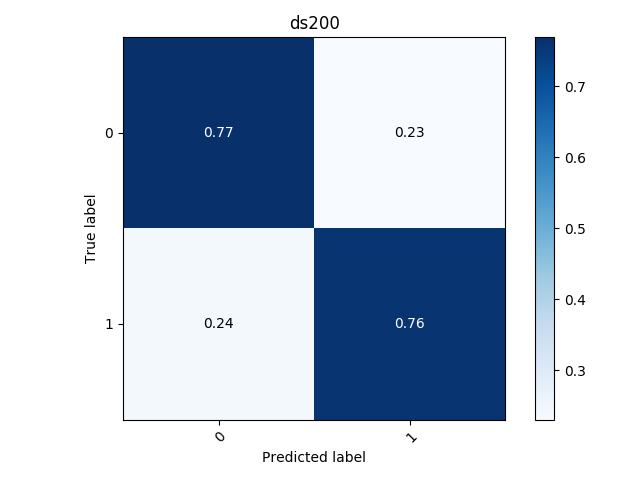
\includegraphics{Figure/confMatr/mtr_ds200.png}
    \caption{matrici di confusione dell'intero dataset}
    \label{fig:mtrconf_sim_200}
\end{figure}
\FloatBarrier

\begin{figure}[h!t]
    \centering
    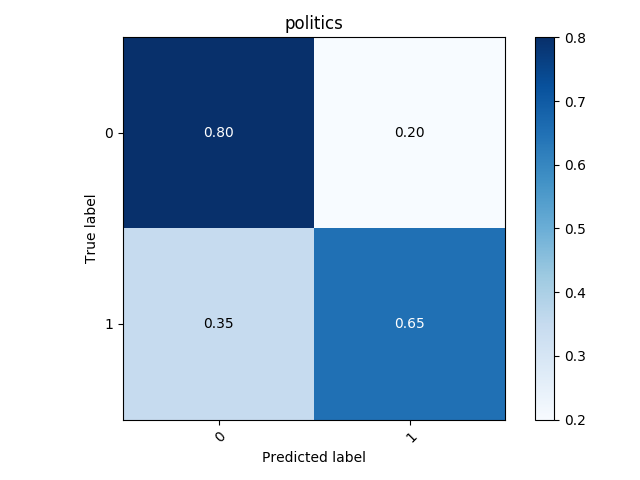
\includegraphics{Figure/confMatr/mtr_politics.png}
    \caption{matrici di confusione del topic politics}
    \label{fig:mtrconf_sim_p}
\end{figure}
\FloatBarrier

\begin{figure}[h!t]
    \centering
    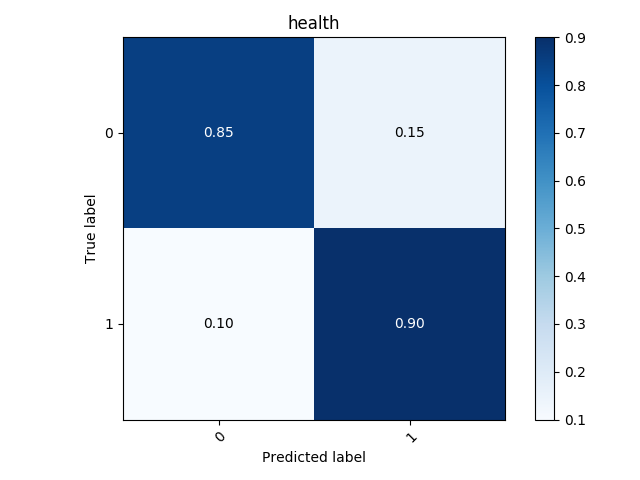
\includegraphics{Figure/confMatr/mtr_health.png}
    \caption{matrici di confusione del topic health}
    \label{fig:mtrconf_sim_h}
\end{figure}
\FloatBarrier

\begin{figure}[h!t]
    \centering
    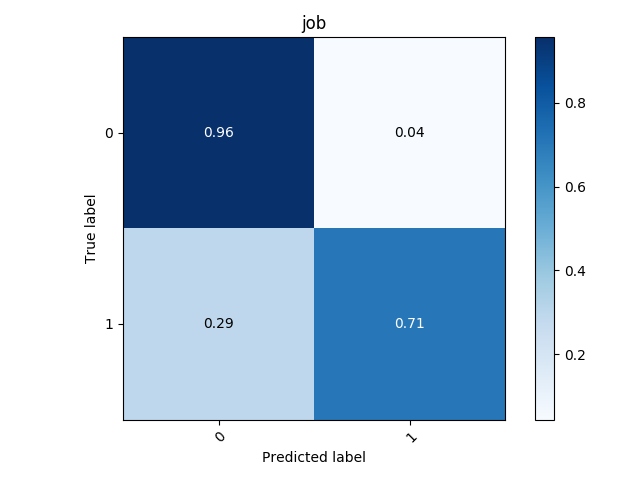
\includegraphics{Figure/confMatr/mtr_job.png}
    \caption{matrici di confusione del topic job}
    \label{fig:mtrconf_sim_j}
\end{figure}
\FloatBarrier


\begin{figure}[h!t]
    \centering
    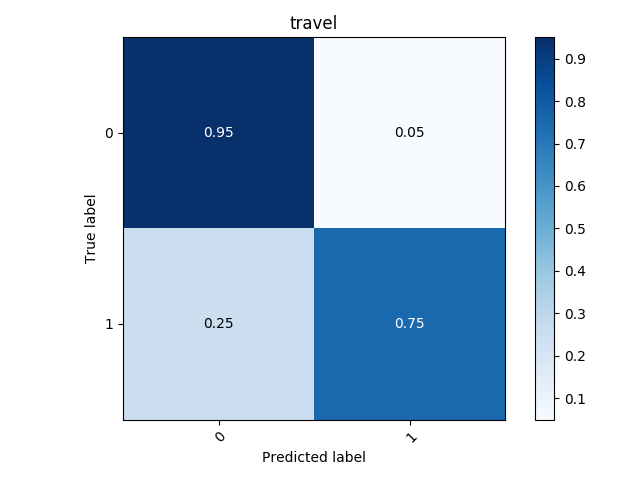
\includegraphics{Figure/confMatr/mtr_travel.png}
    \caption{matrici di confusione del topic travel}
    \label{fig:mtrconf_sim_t}
\end{figure}
\FloatBarrier


\begin{figure}[h!t]
    \centering
    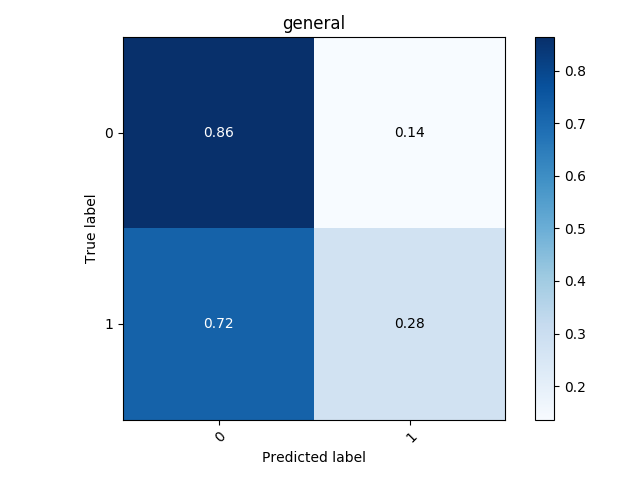
\includegraphics{Figure/confMatr/mtr_general.png}
    \caption{matrici di confusione del topic general}
    \label{fig:mtrconf_sim_g}
\end{figure}
\FloatBarrier

\begin{thebibliography}{9}
\bibitem{looseTweets} 
Huina Mao, Xin Shuaiand Apu Kapadia.\newline
\textit{Loose Tweets: An Analysis of Privacy Leaks on Twitter}. \newline
WPES 2011.

\bibitem{privacyDetective}
Aylin Caliskan, Jonathan Walsh, Rachel Greenstadt.\newline
\textit{Privacy Detective: Detecting Private Information and Collective Privacy Behavior in a Large Social Network}.\newline
WPES 2014

\bibitem{dontTweetThis}
Qiaozhi Wang, Hao Xue, Fengjun Li, Dongwon Lee, and Bo Luo.\newline
\textit{\#DontTweetThis: Scoring Private Information in Social Networks}. \newline
POPETS 2019
\end{thebibliography}
\listoffigures %elenco figure
\listoftables %elenco tabelle
\end{document}
